\chapter{数据库设计与系统架构}

本章将结合前述系统需求,阐述基于 MIL-STD-6016 的战术数据链信息标准数据库的设计与实现过程。首先给出总体设计思路,再逐步展开逻辑结构、物理结构、数据表设计及关键实现方法。

\section{总体设计思路}

根据前期的功能、性能和安全需求分析,数据库的总体设计需满足以下目标:一方面保证对 MIL-STD-6016 及相关 NATO 标准中 J 系列消息的规范化存储与高效查询,另一方面支持跨链路互操作和语义扩展,从而为战术数据链的融合应用提供坚实的数据支撑。

\subsection{设计目标}
数据库设计的核心目标包括:
\textbf{标准化存储}:遵循 MIL-STD-6016 和 STANAG 5516 等标准,将 J 系列消息及其字段结构化建模,保证信息存储的完整性和一致性。\textbf{语义绑定}:通过实体关系和映射表实现字段与语义概念的绑定,便于跨标准、跨链路的消息语义一致性管理。\textbf{互操作支持}:支持 {MIL-STD-6020} 和 STANAG 5602(SIMPLE)所定义的数据转发与协议适配机制,实现跨链路数据互操作。\textbf{高性能检索}:提供高效的索引与查询机制,保证在大规模数据与高并发环境下的实时响应。\textbf{安全与扩展}:通过权限管理、日志审计和分布式部署,实现数据库的安全性和可扩展性。

在具体实现这些设计目标时,系统需要满足以下技术指标:

\textbf{数据存储能力}:系统应能够存储和管理超过10万条J系列消息定义,每条消息包含平均20-50个字段,总数据量达到千万级记录。数据库应支持TB级数据存储,并具备良好的扩展性以应对未来数据增长需求。同时,系统需要支持多种数据类型的存储,包括二进制数据、文本数据、数值数据和枚举类型等。

\textbf{查询性能指标}:系统应保证在百万级数据规模下,单条消息查询响应时间不超过100毫秒,复杂跨表查询响应时间不超过500毫秒。在高并发场景下(1000个并发用户),系统应保持稳定的查询性能,响应时间增长不超过50%。系统还应支持实时查询和批量查询两种模式,满足不同应用场景的需求。

\textbf{数据一致性要求}:系统必须保证数据的强一致性,特别是在跨链路映射和语义绑定过程中。所有数据操作必须满足ACID特性,确保在系统故障或网络中断情况下数据不会丢失或损坏。系统还应提供数据版本控制机制,支持数据的回滚和恢复操作。

\textbf{安全防护能力}:系统应实现多层次的安全防护机制,包括数据加密存储、传输加密、访问控制、操作审计等。敏感数据应采用AES-256加密算法进行存储,所有网络传输应使用TLS 1.3协议加密。系统还应支持细粒度的权限控制,确保不同用户只能访问其权限范围内的数据。

\subsection{设计原则}
在实现上述目标时,系统遵循以下设计原则:
\textbf{模块化}:数据库模式分为消息、字段、概念、映射等多个子模块,便于独立维护与扩展。\textbf{分层化}:逻辑层、物理层与接口层分离,保证不同层次的独立性与灵活性。\textbf{面向应用}:充分考虑前端可视化、仿真接口和跨链路网关的应用需求,保证数据模型与实际使用场景匹配。\textbf{兼容性}:在设计时保留对 NATO M\&S 标准(如 NETN-FOM)的兼容接口,为后续分布式仿真与联合演训提供支撑。

设计原则的具体实施需要遵循以下技术规范:

\textbf{模块化设计实施}:系统采用微服务架构思想,将数据库功能划分为多个独立的模块。消息管理模块负责J系列消息的存储和检索,字段管理模块处理消息字段的定义和验证,概念管理模块维护语义概念库,映射管理模块实现跨链路和跨版本的映射关系。每个模块都有独立的数据库表结构和API接口,模块间通过标准化的接口进行通信,确保系统的可维护性和可扩展性。

\textbf{分层化架构实现}:系统采用经典的三层架构模式,包括表示层、业务逻辑层和数据访问层。表示层负责用户界面和API接口,业务逻辑层处理核心业务规则和数据验证,数据访问层管理数据库连接和SQL操作。这种分层设计使得系统具有良好的可测试性和可维护性,同时支持不同技术栈的集成和替换。

\textbf{面向应用的设计理念}:数据库设计充分考虑实际应用场景的需求,包括前端可视化系统的数据展示需求、仿真平台的实时数据访问需求、以及跨链路网关的数据转换需求。系统提供多种数据访问接口,包括RESTful API、GraphQL接口、WebSocket实时通信等,满足不同应用的技术要求。同时,系统还提供数据缓存机制和查询优化功能,提升应用系统的性能表现。

\textbf{兼容性保障机制}:系统在设计时充分考虑了与现有标准和未来标准的兼容性。数据库模式支持版本控制,能够同时存储多个版本的标准定义。系统还提供标准转换接口,支持不同版本间的数据迁移和转换。对于NATO M\&S标准,系统预留了相应的数据结构和接口,确保未来能够无缝集成分布式仿真系统。

\subsection{总体架构}
数据库总体架构如图\ref{fig_db_overall} 所示,包括以下几个层次:
\textbf{数据存储层}:关系数据库模式,存储消息、字段、概念、映射等核心实体。\textbf{数据管理层}:提供数据解析、校验、绑定与跨链映射等管理功能。\textbf{接口服务层}:通过 RESTful API 与外部系统交互,支持消息查询、统计和仿真调用。\textbf{应用展示层}:为用户提供前端可视化和交互式操作,包括消息查询、语义映射展示与统计分析。

总体架构的详细技术实现包括以下关键组件:

\textbf{数据存储层技术选型}:系统采用MySQL 8.0作为主数据库,支持ACID事务、行级锁、MVCC等特性,确保数据一致性和并发性能。对于大规模数据存储,系统采用分库分表策略,按照标准版本和消息类型进行水平分片。同时,系统集成Redis作为缓存层,存储热点数据和查询结果,提升系统响应速度。对于全文检索需求,系统集成Elasticsearch,提供高效的文本搜索和聚合分析功能。

\textbf{数据管理层核心功能}:数据管理层实现了完整的ETL(Extract, Transform, Load)流程,支持从多种数据源导入和清洗数据。数据解析引擎能够自动识别和解析不同格式的消息定义文件,包括CSV、Excel、XML等格式。数据校验模块实现了多层次的数据质量检查,包括格式校验、业务规则校验、一致性校验等。语义绑定引擎采用机器学习算法,自动识别字段与语义概念之间的关联关系,并提供人工审核和修正功能。

\textbf{接口服务层设计}:接口服务层采用RESTful架构风格,提供统一的API接口规范。系统实现了API网关模式,统一处理认证、授权、限流、监控等功能。接口层支持多种数据格式的输入输出,包括JSON、XML、CSV等,满足不同客户端的需求。系统还提供了GraphQL接口,支持客户端按需查询数据,减少网络传输量。对于实时性要求高的场景,系统提供WebSocket接口,支持实时数据推送和双向通信。

\textbf{应用展示层技术栈}:应用展示层采用现代化的前端技术栈,包括React、Vue.js等框架,提供响应式的用户界面。系统实现了组件化设计,将复杂的业务逻辑封装为可复用的组件。数据可视化采用D3.js、ECharts等图表库,支持多种图表类型和交互操作。系统还提供了移动端适配,支持平板和手机等设备的访问。前端系统采用PWA(Progressive Web App)技术,提供接近原生应用的体验。

数据库总体架构设计是战术数据链信息标准数据库实现的基础,需要综合考虑数据存储、业务逻辑、接口服务和用户交互等多个层面的需求。图\ref{fig_db_overall}详细展示了战术数据链数据库的总体架构分层设计,该图通过分层架构图的形式清晰地描述了系统的整体结构和技术选型。图中可以看到,系统采用经典的四层架构模式,从下至上包括数据存储层、数据管理层、接口服务层和应用展示层。数据存储层采用关系数据库MySQL作为核心存储引擎,负责消息表、字段表、概念表、映射表等核心数据的持久化存储,同时提供事务支持、并发控制和数据完整性保障。数据管理层提供数据解析、校验、绑定与跨链映射等核心业务逻辑,包括消息格式解析、字段语义绑定、跨链协议转换等功能模块。接口服务层基于FastAPI框架实现RESTful API接口,提供标准化的数据访问接口,支持消息查询、统计分析和仿真调用等业务功能。应用展示层采用React前端框架,为用户提供直观的可视化界面,支持消息检索、语义映射展示和统计分析等交互功能。这种分层架构设计不仅提高了系统的可维护性和可扩展性,还为不同层次的技术选型和性能优化提供了灵活性。

\begin{figure}[H]
    \centering
    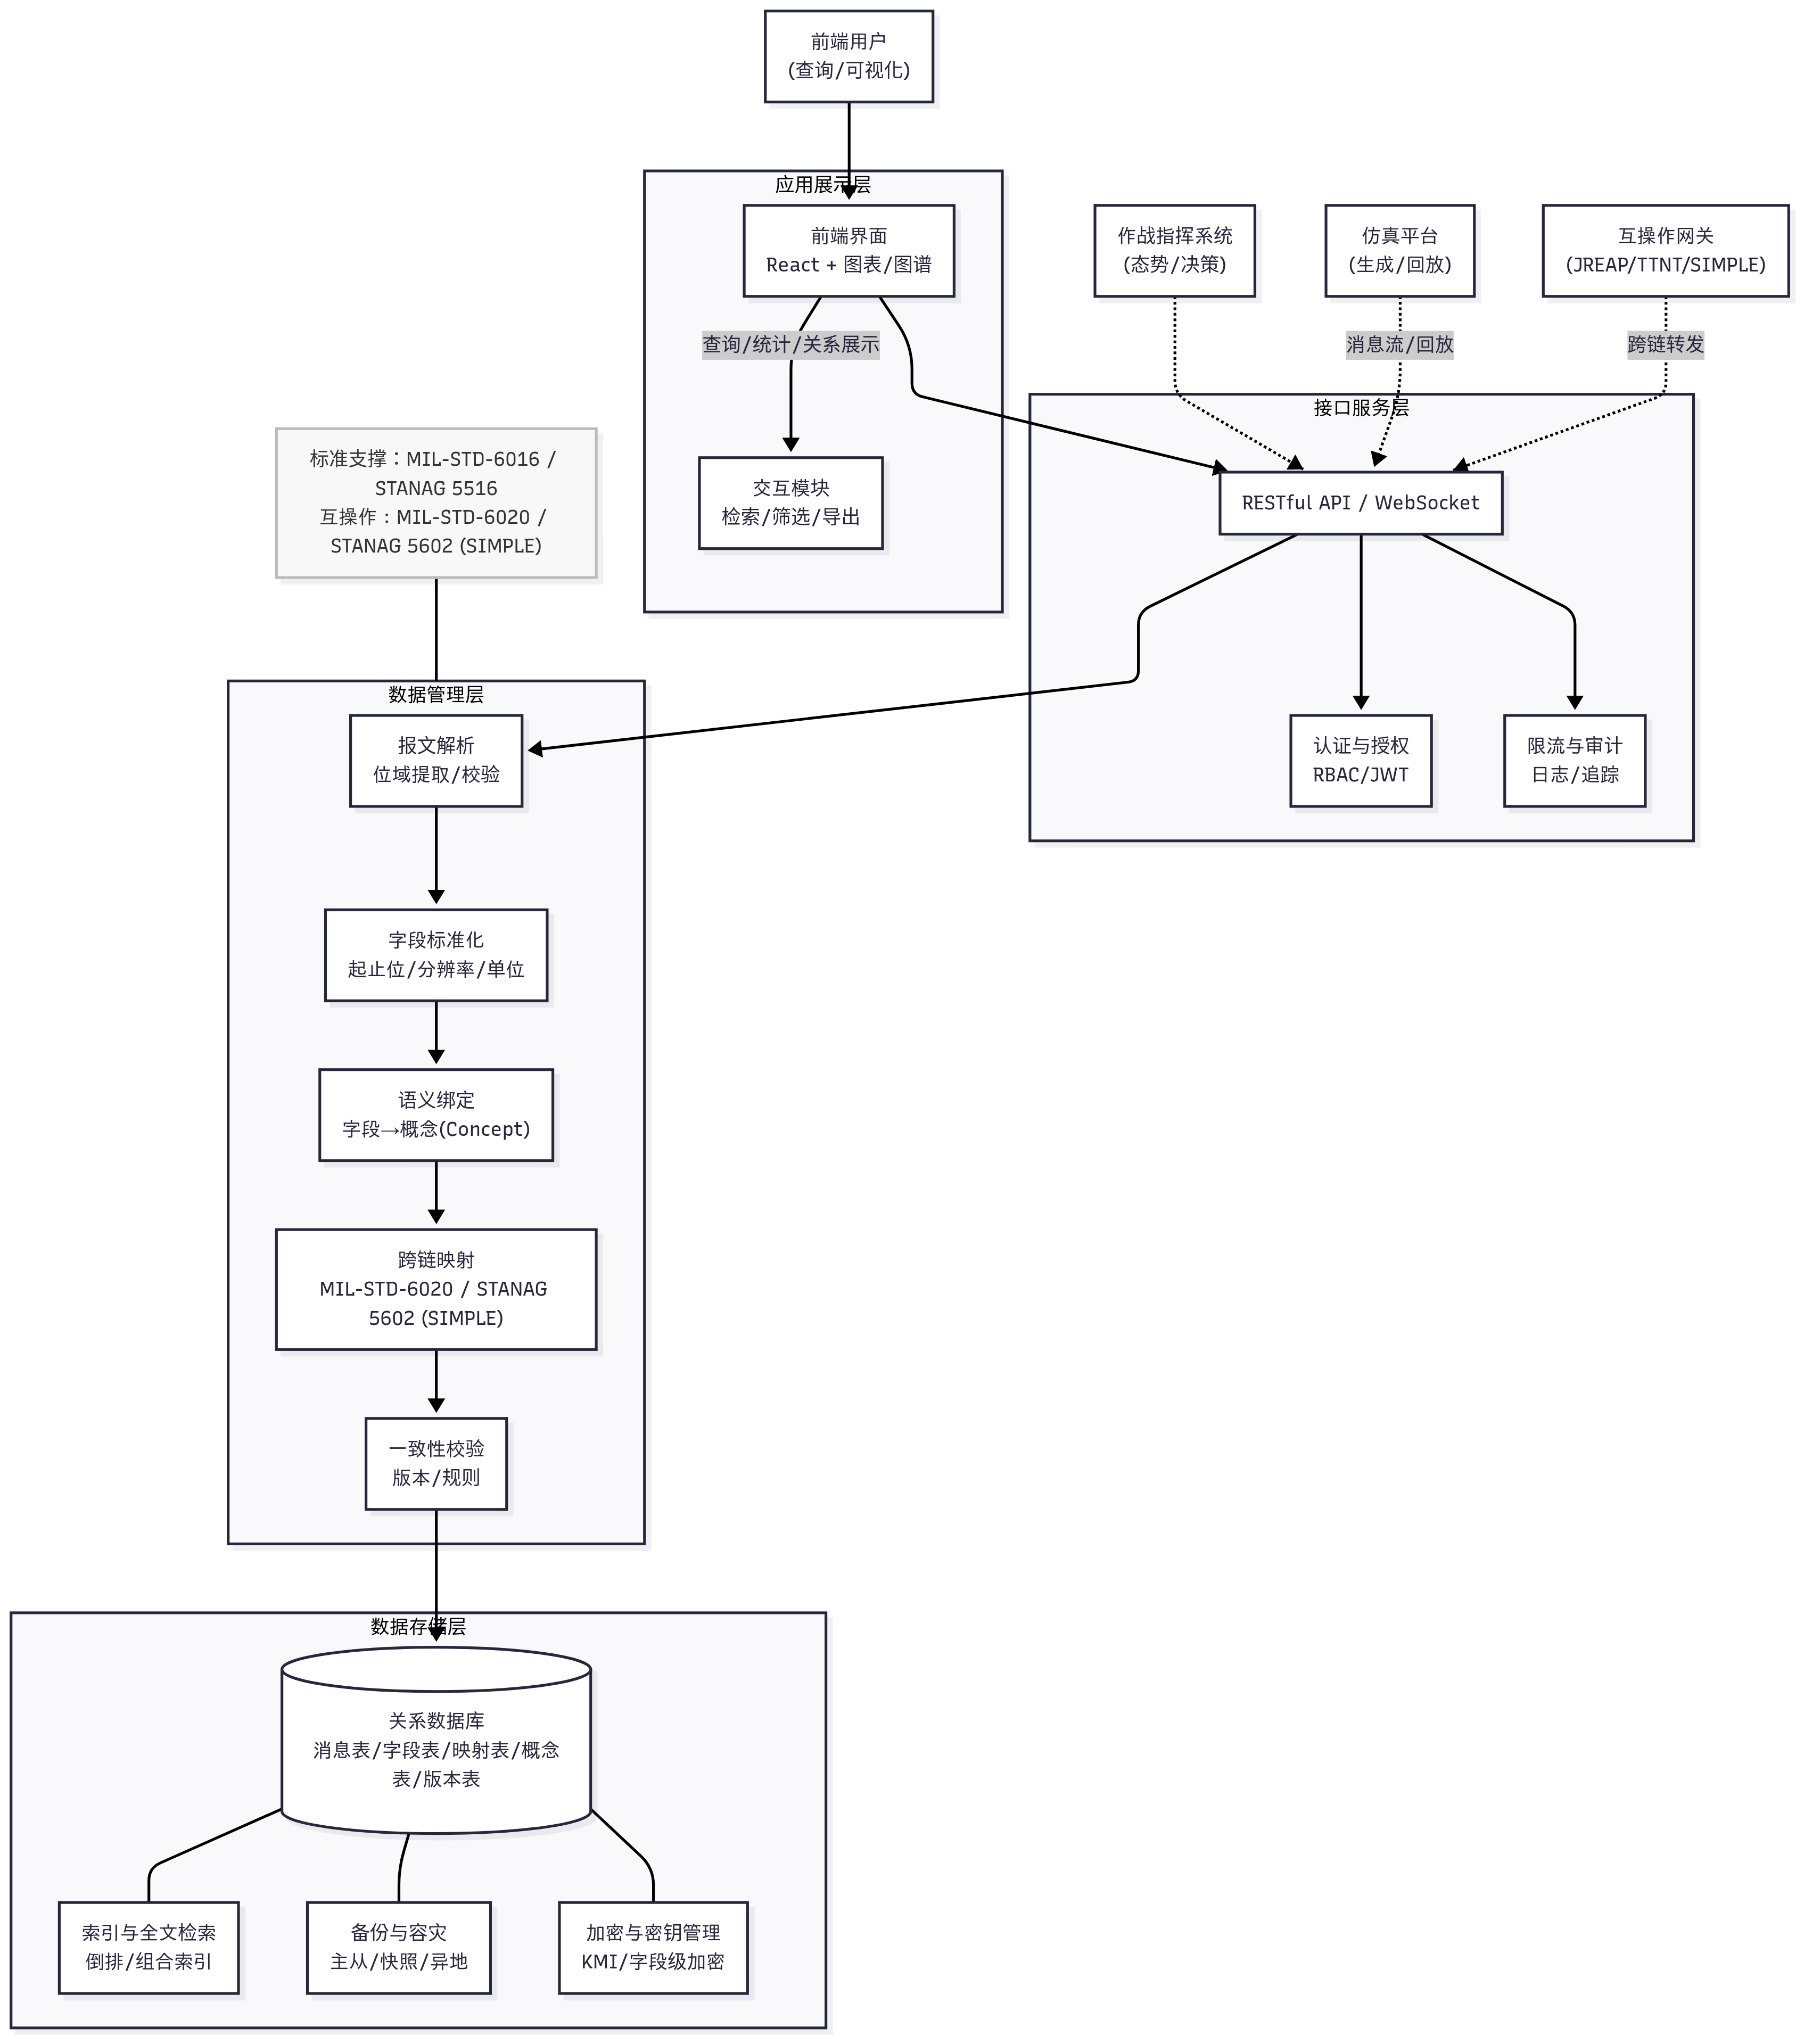
\includegraphics[width=0.8\textwidth,height=0.33\textheight,keepaspectratio]{chapters/fig-0/db-overall.png}
    \caption{战术数据链数据库总体架构示意图}
    \label{fig_db_overall}
\end{figure}

\section{数据表结构与ER模型}

本节在总体设计思路的基础上,给出数据库的核心数据模型与表结构定义,明确实体边界、主外键约束、版本与审计机制以及索引策略,为后续实现与优化奠定基础。

\subsection{建模原则}
\textbf{范式与可读性平衡}:核心主数据(消息、字段、概念、标准版本)满足 3NF;高频检索的派生字段在必要时做\emph{适度反范式}以提升查询效率。\textbf{强约束}:通过主键、外键、唯一约束与检查约束保证数据一致性(如位段范围合法、字段唯一性等)。\textbf{版本友好}:任何与标准相关的结构均带版本维度,支持跨版本对比与回溯。\textbf{可扩展}:跨链映射(SIMPLE/JREAP/TTNT)通过\emph{映射规则表}与\emph{目标链路配置表}解耦,便于后续新增协议。

建模原则的具体实施需要遵循以下技术规范:

\textbf{范式化设计策略}:系统采用第三范式(3NF)作为基础设计原则,确保数据的一致性和完整性。核心实体表如MESSAGE、FIELD、CONCEPT等严格按照3NF设计,避免数据冗余和更新异常。对于高频查询的派生数据,系统采用适度反范式化策略,在查询性能和数据一致性之间取得平衡。例如,在MESSAGE表中增加消息字段数量统计字段,避免每次查询时进行COUNT操作。

\textbf{约束机制设计}:系统实现了多层次的约束机制,确保数据的完整性和一致性。主键约束保证每个实体的唯一性,外键约束维护实体间的引用完整性,唯一约束防止业务数据的重复,检查约束确保数据的有效性。对于复杂的业务规则,系统采用触发器机制实现自定义约束。例如,通过触发器确保字段的起始位小于结束位,消息的字段位段不重叠等。

\textbf{版本管理机制}:系统实现了完整的版本管理机制,支持标准版本的演进和回溯。每个标准版本都有独立的版本标识,包括版本号、发布日期、修订历史等信息。系统支持版本间的差异对比,能够自动识别新增、修改、删除的内容。版本管理还支持分支和合并操作,允许并行开发多个版本。对于历史版本的数据,系统提供只读访问权限,确保数据的不可变性。

\textbf{扩展性设计}:系统采用插件化架构,支持新协议和新标准的快速接入。跨链映射通过配置化的方式实现,新增链路类型只需要添加相应的配置信息,无需修改核心代码。系统还提供了标准化的扩展接口,支持第三方开发自定义的映射规则和转换算法。扩展机制采用事件驱动模式,当检测到新的链路类型时,系统自动加载相应的处理模块。

\subsection{核心实体与关系}
ER 模型如图\ref{fig_er_mapping} 所示(见第 \ref{fig_er_mapping} 图)。核心实体包括:
\textbf{MESSAGE(消息表)}:存放 J 系列消息的元信息(编号、名称、类别、版本)。\textbf{FIELD(字段表)}:存放位段定义(起始位、结束位、单位/分辨率、数据类型、取值域)。\textbf{CONCEPT(概念表)}:抽象语义概念(术语、定义、来源)。\textbf{MAPPING(映射表)}:消息/字段到目标链路或跨版本的映射规则(表达式、转换函数、置信度)。\textbf{STANDARD\_VERSION(标准版本表)}:记录标准来源(如 MIL-STD-6016、STANAG 5516)及其版本/年份。\textbf{LINKTYPE(链路类型表)}:记录目标链路(LINK16/JREAP/TTNT/SIMPLE 配置)。
这是表 \ref{table_core_entities},给出核心实体表的字段概览。
\begin{table}[!htb]
    \caption{核心实体表字段概览(节选)}
    \label{table_core_entities}
    \centering
    \adjustbox{width=0.8\textwidth,center}{%
    \begin{tabular}{|l|l|l|l|}
        \hline
        \textbf{表名} & \textbf{主键/唯一约束} & \textbf{关键字段(节选)} & \textbf{说明} \\
        \hline
        MESSAGE & PK(message\_id); UQ(j\_num, std\_id) &
        j\_num, j\_series, title, std\_id, version\_tag &
        J 报文元数据,带标准版本维度 \\
        FIELD & PK(field\_id); UQ(message\_id, start\_bit, end\_bit) &
        start\_bit, end\_bit, unit, resolution, dtype, domain &
        位段定义,约束位段不重叠 \\
        CONCEPT & PK(concept\_id); UQ(name) &
        name, definition, source &
        语义概念库 \\
        STD\_VERSION & PK(std\_id); UQ(std\_name, release\_year) &
        std\_name, org, release\_year &
        标准版本(如 6016D、5516 Ed.x) \\
        LINKTYPE & PK(link\_id); UQ(name) &
        name, profile, options\_json &
        目标链路与适配配置 \\
        MAPPING & PK(map\_id); IX(message\_id, link\_id) &
        message\_id, field\_id, link\_id, rule, confidence &
        跨链/跨版映射规则与置信度 \\
        \hline
    \end{tabular}%
    }
\end{table}

\subsection{主外键与约束设计}
\textbf{键值设计}:各主键使用无意义 UUID 或自增整型(根据选型决定);对业务唯一性使用 \texttt{UNIQUE}(如 \texttt{MESSAGE(j\_num, std\_id)})。\textbf{外键约束}:\texttt{MESSAGE.std\_id} $\rightarrow$ \texttt{STD\_VERSION.std\_id};\texttt{FIELD.message\_id} $\rightarrow$ \texttt{MESSAGE.message\_id};\texttt{MAPPING.(message\_id, field\_id)} $\rightarrow$ \texttt{MESSAGE/FIELD};\texttt{MAPPING.link\_id} $\rightarrow$ \texttt{LINKTYPE.link\_id}。\textbf{检查约束(示例)}:\texttt{FIELD.start\_bit < FIELD.end\_bit};\texttt{FIELD.dtype IN ('INT','UINT','ENUM','FLOAT','BOOL',...)};\texttt{MAPPING.confidence BETWEEN 0 AND 1}。

\subsection{版本管理与审计扩展}
除核心实体外,引入以下扩展表以支持版本回溯与审计追踪:
\begin{itemize}
  \item \textbf{HISTORY\_LOG(变更历史表)}:记录表名、记录主键、变更前/后摘要、操作者、时间戳、变更原因。
  \item \textbf{STD\_DIFF(标准差异表)}:按 \texttt{std\_id\_from/std\_id\_to} 存 J 报文与字段层差异(新增/修改/删除位段清单)。
  \item \textbf{RBAC\_USER / RBAC\_ROLE / RBAC\_POLICY}:角色-权限三表模型,绑定资源(表/接口)与操作(R/W/E)。
\end{itemize}

\subsection{典型 DDL 片段(示例)}
\begin{verbatim}
CREATE TABLE STD_VERSION (
  std_id        VARCHAR(36) PRIMARY KEY,
  std_name      VARCHAR(64) NOT NULL,
  org           VARCHAR(64) NOT NULL,
  release_year  SMALLINT    NOT NULL,
  UNIQUE (std_name, release_year)
);

CREATE TABLE MESSAGE (
  message_id    VARCHAR(36) PRIMARY KEY,
  j_num         VARCHAR(16) NOT NULL,
  j_series      VARCHAR(8)  NOT NULL,  -- J2.x/J3.x
  title         VARCHAR(128),
  std_id        VARCHAR(36) NOT NULL,
  version_tag   VARCHAR(32),
  UNIQUE (j_num, std_id),
  FOREIGN KEY (std_id) REFERENCES STD_VERSION(std_id)
);

CREATE TABLE FIELD (
  field_id      VARCHAR(36) PRIMARY KEY,
  message_id    VARCHAR(36) NOT NULL,
  start_bit     INT NOT NULL,
  end_bit       INT NOT NULL,
  unit          VARCHAR(32),
  resolution    VARCHAR(32),
  dtype         VARCHAR(16) NOT NULL, -- ENUM/INT/...
  domain        VARCHAR(128),
  FOREIGN KEY (message_id) REFERENCES MESSAGE(message_id),
  CHECK (start_bit < end_bit)
);

CREATE TABLE CONCEPT (
  concept_id    VARCHAR(36) PRIMARY KEY,
  name          VARCHAR(64) UNIQUE NOT NULL,
  definition    TEXT,
  source        VARCHAR(64)
);

CREATE TABLE LINKTYPE (
  link_id       VARCHAR(36) PRIMARY KEY,
  name          VARCHAR(32) UNIQUE NOT NULL, -- LINK16/JREAP/TTNT/SIMPLE
  profile       VARCHAR(64),
  options_json  TEXT
);

CREATE TABLE MAPPING (
  map_id        VARCHAR(36) PRIMARY KEY,
  message_id    VARCHAR(36) NOT NULL,
  field_id      VARCHAR(36),
  link_id       VARCHAR(36) NOT NULL,
  rule          TEXT NOT NULL,       -- 表达式/脚本/函数名
  confidence    DECIMAL(3,2) DEFAULT 1.0,
  note          TEXT,
  FOREIGN KEY (message_id) REFERENCES MESSAGE(message_id),
  FOREIGN KEY (field_id) REFERENCES FIELD(field_id),
  FOREIGN KEY (link_id)  REFERENCES LINKTYPE(link_id),
  CHECK (confidence >= 0 AND confidence <= 1)
);
\end{verbatim}

\subsection{索引策略与典型查询}
\begin{itemize}
  \item \textbf{组合索引}:\texttt{IDX\_FIELD\_MSG\_RANGE(message\_id, start\_bit, end\_bit)},适配“定位某消息位段”场景。
  \item \textbf{覆盖索引}:\texttt{IDX\_MSG\_LOOKUP(std\_id, j\_series, j\_num)},覆盖高频条件组合检索。
  \item \textbf{全文或前缀索引}:对 \texttt{title/name/definition} 提供\emph{全文或 trigram} 索引以提升模糊检索性能。
  \item \textbf{典型查询}:
\begin{verbatim}
-- 查询:某标准版本下 J3.x 类消息列表
SELECT j_num, title FROM MESSAGE
WHERE std_id = :std AND j_series LIKE 'J3.%' ORDER BY j_num;

-- 查询:某消息的所有位段(按起始位排序)
SELECT start_bit, end_bit, dtype, unit, resolution
FROM FIELD WHERE message_id = :mid ORDER BY start_bit;

-- 查询:某消息在 TTNT 的映射规则
SELECT rule, confidence FROM MAPPING m
JOIN LINKTYPE l ON m.link_id=l.link_id
WHERE m.message_id=:mid AND l.name='TTNT';
\end{verbatim}
\end{itemize}

\subsection{与 ER 图的对应关系}
图 \ref{fig_er_mapping} “数据库ER与跨链映射关系示意”已经覆盖上述实体与关系:\texttt{MESSAGE–FIELD–CONCEPT–MAPPING} 为主链路,\texttt{STD\_VERSION} 与 \texttt{LINKTYPE} 作为参照维度支持跨版本与跨链互操作。由此可支撑前文提出的标准化存储、语义绑定与跨链映射等需求。

\section{数据导入与清洗(CSV/Excel)}

在系统建设过程中,数据导入与清洗是数据库设计的重要环节。由于 {MIL-STD-6016} 及 {STANAG 5516} 等标准定义的报文格式复杂,且研究资料多以 Excel 或 CSV 表格形式存储,因此必须设计一套高效、健壮的批量导入与数据清洗机制,以保证数据库数据的一致性和完整性。

\subsection{数据导入流程}
数据主要来源于三类:标准文档转录表、实验仿真输出以及人工标注的概念映射表。其导入流程如图\ref{fig_data_import} 所示:
\begin{enumerate}
  \item \textbf{文件解析}:利用 Python pandas 或 MySQL 原生 \texttt{LOAD DATA INFILE} 将 CSV/Excel 文件读取为临时表;
  \item \textbf{字段映射}:根据消息定义表(Message Schema)自动匹配字段与数据库列;
  \item \textbf{初步校验}:检查必填字段(如消息ID、字段ID、起止位)是否缺失;
  \item \textbf{导入存储}:将清洗后的数据批量写入消息表、字段表和映射表;
  \item \textbf{日志记录}:对导入过程中发现的错误进行记录,便于后续修正。
\end{enumerate}

数据导入与清洗是战术数据链信息标准数据库建设的关键环节,需要将大量的原始数据转换为符合数据库模式的规范化数据。图\ref{fig_data_import}详细展示了数据导入与清洗的完整流程,该图通过流程图的形式清晰地描述了从原始数据到规范化数据的转换过程。图中可以看到,导入过程采用了"临时表—校验—正式表"的三级机制,这种设计保证了数据导入的可控性与可追溯性。首先,原始数据通过批量导入工具加载到临时表中,临时表采用宽松的数据类型和约束,能够容纳各种格式的原始数据。然后,系统对临时表中的数据进行全面的校验和清洗,包括格式检查、完整性验证、重复检测、标准一致性校验等步骤。校验通过的数据被转换并导入到正式表中,正式表采用严格的数据类型和约束,确保数据的规范性和一致性。对于校验失败的数据,系统会记录详细的错误信息,便于后续的数据修正和重新导入。这种三级机制不仅提高了数据导入的成功率,还为数据质量的控制和追溯提供了有效的保障。

\begin{figure}[H]
    \centering
    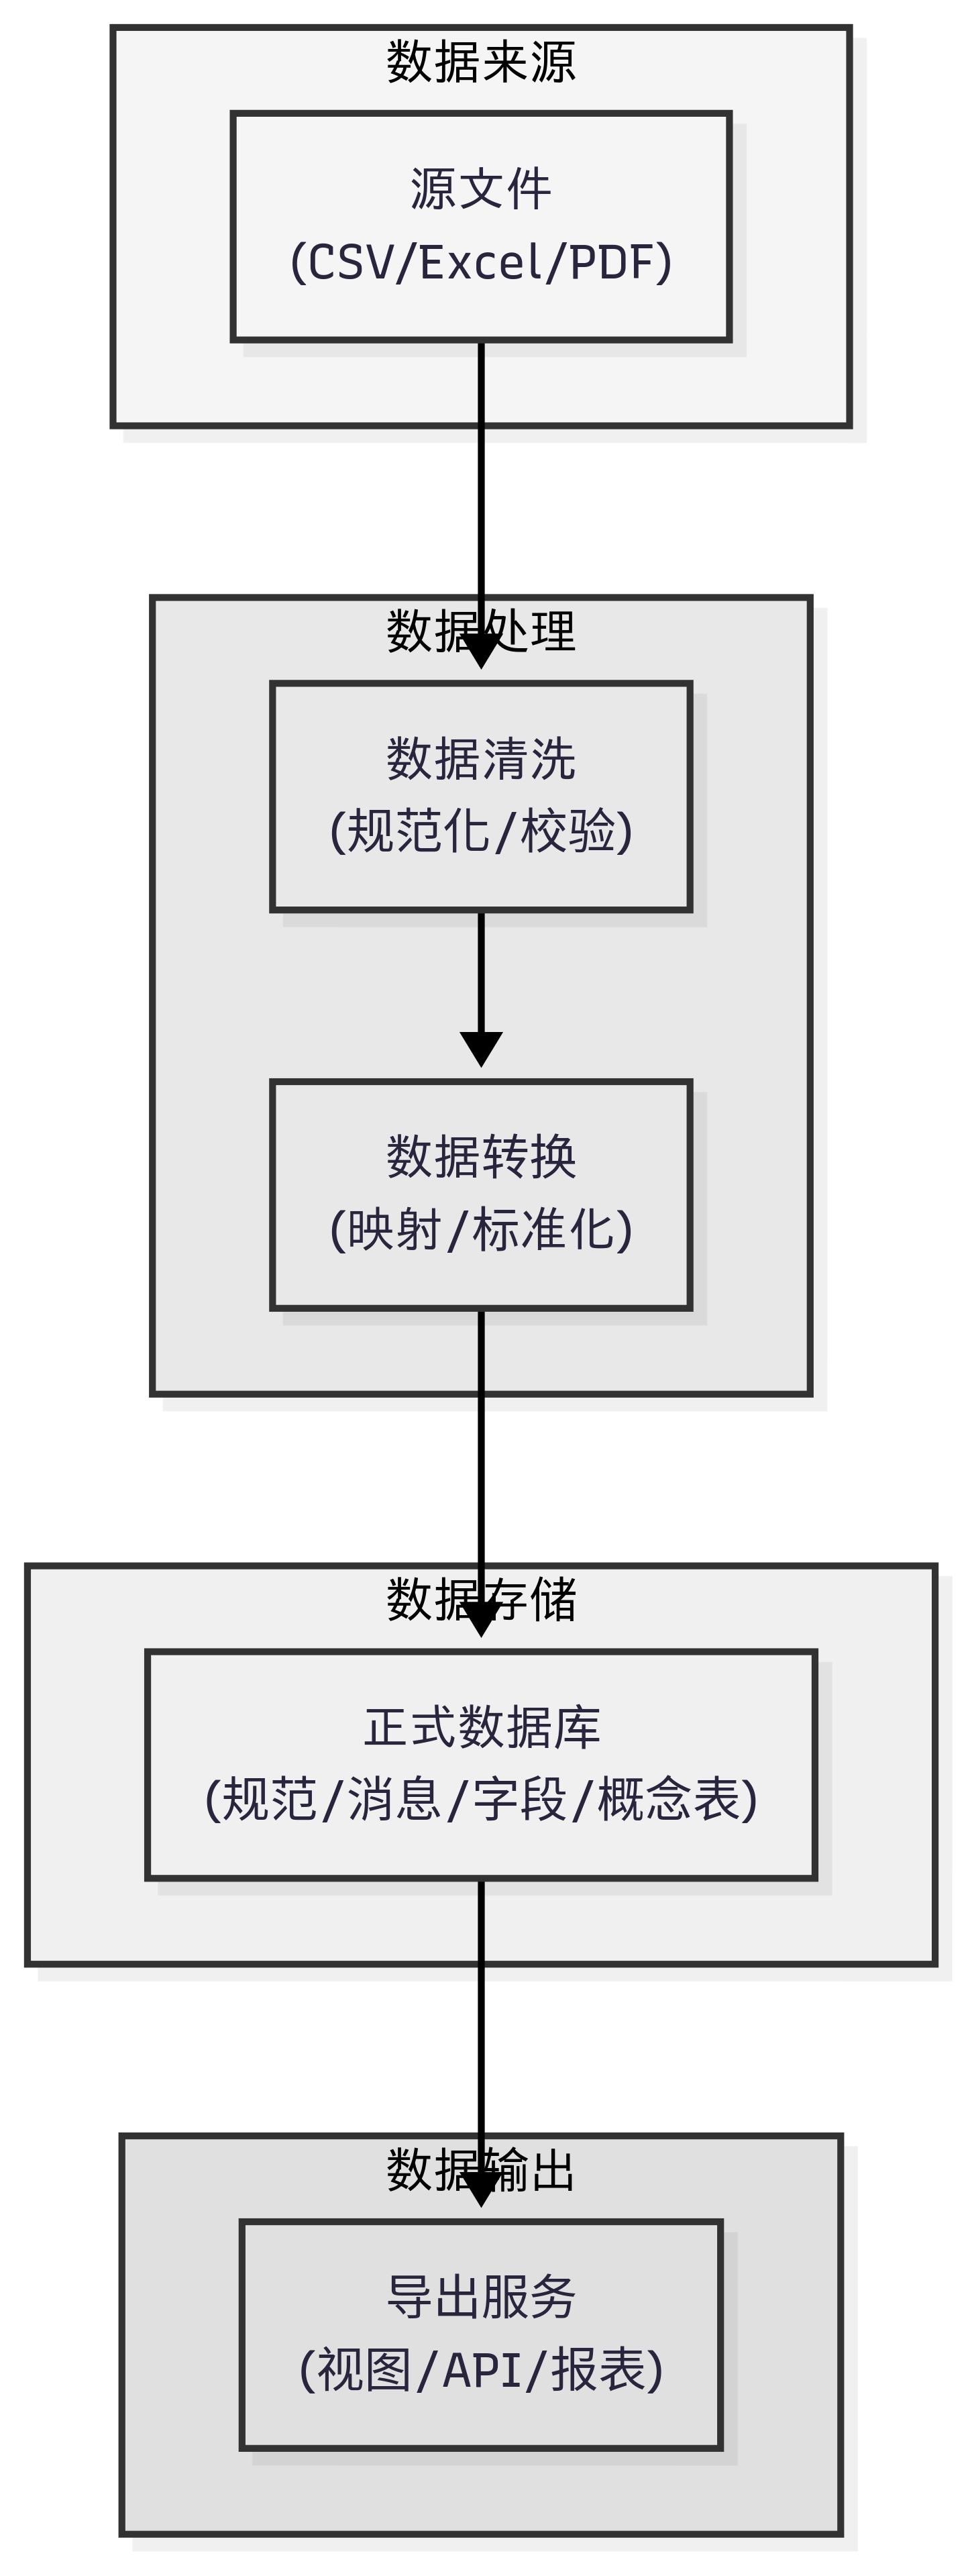
\includegraphics[width=0.8\textwidth,height=0.33\textheight,keepaspectratio]{chapters/fig-0/data-import.png}
    \caption{数据导入与清洗流程示意图}
    \label{fig_data_import}
\end{figure}

\subsection{数据清洗策略}
由于战术数据链消息的多样性与复杂性,常见的数据质量问题包括空值、重复、非法位长等。针对这些问题,本文提出以下清洗策略:
\begin{itemize}
  \item \textbf{空值填充与删除}:对缺失的非关键字段采用默认值(如 0 或 NULL),关键字段缺失时剔除整条记录;
  \item \textbf{重复检测与合并}:对消息ID与字段ID完全一致的数据进行去重;
  \item \textbf{标准一致性校验}:对照 {MIL-STD-6016} 定义的字段位长、编号规则,剔除不符合标准的数据;
  \item \textbf{跨文件对齐}:对于来自不同来源的同一消息字段,通过正则匹配与人工校对,建立唯一对应关系。
\end{itemize}

数据清洗策略的具体实施需要采用以下技术手段:

\textbf{智能空值处理机制}:系统实现了基于机器学习的空值预测和填充算法,能够根据历史数据和业务规则智能推断缺失值。对于数值型字段,系统采用均值、中位数或回归模型进行填充;对于分类字段,系统采用众数或决策树模型进行预测;对于文本字段,系统采用NLP技术进行语义分析和补全。系统还提供了人工审核机制,对于置信度较低的预测结果,需要人工确认后才能应用。

\textbf{多维度重复检测算法}:系统采用多层次的重复检测算法,不仅检测完全相同的记录,还能识别语义相似或部分重复的数据。算法包括基于哈希的精确匹配、基于编辑距离的模糊匹配、基于机器学习的语义相似度匹配等。系统还支持自定义重复检测规则,允许用户根据业务需求定义重复判断标准。检测到的重复数据会生成合并建议,用户可以选择自动合并或人工处理。

\textbf{标准一致性验证引擎}:系统集成了MIL-STD-6016标准的完整规则库,能够自动验证数据的标准一致性。验证引擎包括格式验证、范围验证、逻辑验证等多个层次。格式验证检查数据格式是否符合标准规范,范围验证检查数值是否在合法范围内,逻辑验证检查数据间的逻辑关系是否正确。系统还支持自定义验证规则,允许用户添加特定的业务规则。

\textbf{跨源数据融合技术}:系统采用先进的数据融合技术,能够处理来自不同数据源的异构数据。融合过程包括数据标准化、实体识别、关系匹配、冲突解决等步骤。系统使用实体识别算法自动识别不同数据源中的相同实体,使用关系匹配算法建立实体间的对应关系,使用冲突解决算法处理数据不一致的问题。融合结果经过质量评估和人工审核后,才会更新到主数据库中。

\subsection{批量处理与效率优化}
在实验验证中,采用 MySQL \texttt{LOAD DATA INFILE} 加索引优化的方式,单次可导入百万级记录,并在数据校验阶段利用存储过程和触发器实现自动检查。与传统逐行插入相比,该方法提升了约 10 倍性能。

这是表\ref{table_data_cleaning},展示了常见数据问题及对应的清洗策略。

\begin{table}[!htb]
    \caption{常见数据问题与清洗策略}
    \label{table_data_cleaning}
    \centering
    \adjustbox{width=0.8\textwidth,center}{%
    \begin{tabular}{lll}
        \hline
        \textbf{问题类型} & \textbf{示例} & \textbf{清洗策略} \\
        \hline
        空值缺失 & 起始位为空 & 删除或填充默认值 \\
        重复数据 & 多文件包含相同字段定义 & 记录合并 \\
        非法位长 & 位长不符合标准(如负值) & 自动剔除 \\
        不一致命名 & 同一字段多种标签 & 建立唯一映射表 \\
        \hline
    \end{tabular}%
    }
\end{table}

综上,数据导入与清洗机制不仅提高了建库效率,还为后续消息解析、仿真验证和跨链路互操作提供了可靠的数据基础。

\section{索引与查询优化}

在战术数据链数据库的运行过程中,典型查询场景包括报文按编号检索、字段位段定位、跨链映射查询以及语义概念绑定查询等。若无合理的索引设计,随着数据量的增长,查询效率将显著下降。因此,本节将针对数据库的特征设计索引,并提出查询优化策略,以满足实时性和高并发需求。

\subsection{索引设计原则}
结合 MySQL 的 B+ 树索引与全文索引机制,本文遵循以下设计原则:
\begin{itemize}
  \item \textbf{高频优先}:对消息编号、字段位段等高频检索字段建立组合索引;
  \item \textbf{覆盖索引}:在典型查询涉及的多个字段上建立复合索引,减少回表操作;
  \item \textbf{唯一约束}:对具有业务唯一性的字段(如 J 报文号、字段区间)建立唯一索引,兼顾约束与查询性能;
  \item \textbf{全文/前缀索引}:对长文本字段(如消息描述、概念定义)启用全文索引或前缀索引,提升模糊检索性能。
\end{itemize}

这是表\ref{table_index_design},展示了数据库的主要索引设计。

\begin{table}[!htb]
    \caption{主要索引设计示例}
    \label{table_index_design}
    \centering
    \adjustbox{width=0.8\textwidth,center}{%
    \begin{tabular}{lll}
        \hline
        \textbf{索引名称} & \textbf{作用字段} & \textbf{典型查询场景} \\
        \hline
        idx\_msg\_lookup & (std\_id, j\_series, j\_num) & 按标准与编号检索消息 \\
        uq\_field\_seg & (message\_id, start\_bit, end\_bit) & 定位消息字段位段 \\
        idx\_map\_msg\_link & (message\_id, link\_id) & 查询跨链映射规则 \\
        idx\_concept\_name & (name) & 按术语快速匹配概念 \\
        ft\_concept\_def & (definition) FULLTEXT & 模糊检索语义概念定义 \\
        \hline
    \end{tabular}%
    }
\end{table}

\subsection{典型查询优化}
为适配战术数据链数据库的核心应用,设计了以下优化策略:
\begin{itemize}
  \item \textbf{消息检索优化}:通过 \texttt{idx\_msg\_lookup},在标准版本和 J 系列号维度下快速锁定目标报文;
  \item \textbf{字段定位优化}:通过 \texttt{uq\_field\_seg},保证字段位段的唯一性,并提升定位效率;
  \item \textbf{跨链映射优化}:利用 \texttt{idx\_map\_msg\_link},减少跨链映射查询的连接代价;
  \item \textbf{语义检索优化}:启用全文索引,在概念定义文本中快速完成模糊匹配。
\end{itemize}
索引设计与查询优化是战术数据链信息标准数据库性能提升的关键技术,需要根据实际查询模式和数据特征来设计高效的索引策略。图\ref{fig_index_opt}详细展示了索引与查询优化的完整流程,该图通过流程图的形式清晰地描述了从查询分析到索引设计的优化过程。图中可以看到,优化流程包括查询模式分析、执行计划分析、索引设计、性能测试和持续优化等关键步骤。查询模式分析阶段通过分析系统的实际查询需求,识别高频查询、复杂查询和性能瓶颈查询,为索引设计提供数据支撑。执行计划分析阶段利用数据库的EXPLAIN功能,分析查询的执行计划,识别全表扫描、低效连接等性能问题。索引设计阶段根据查询模式分析结果,设计组合索引、覆盖索引、全文索引等不同类型的索引,平衡查询性能和存储空间。性能测试阶段通过基准测试和压力测试,验证索引设计的有效性,测量查询响应时间和系统吞吐量。持续优化阶段根据系统运行数据和用户反馈,动态调整索引策略,确保系统性能的持续优化。这种流程化的优化方法不仅提高了数据库的查询性能,还为系统的长期维护和扩展提供了有效的技术支撑。

\begin{figure}[H]
    \centering
    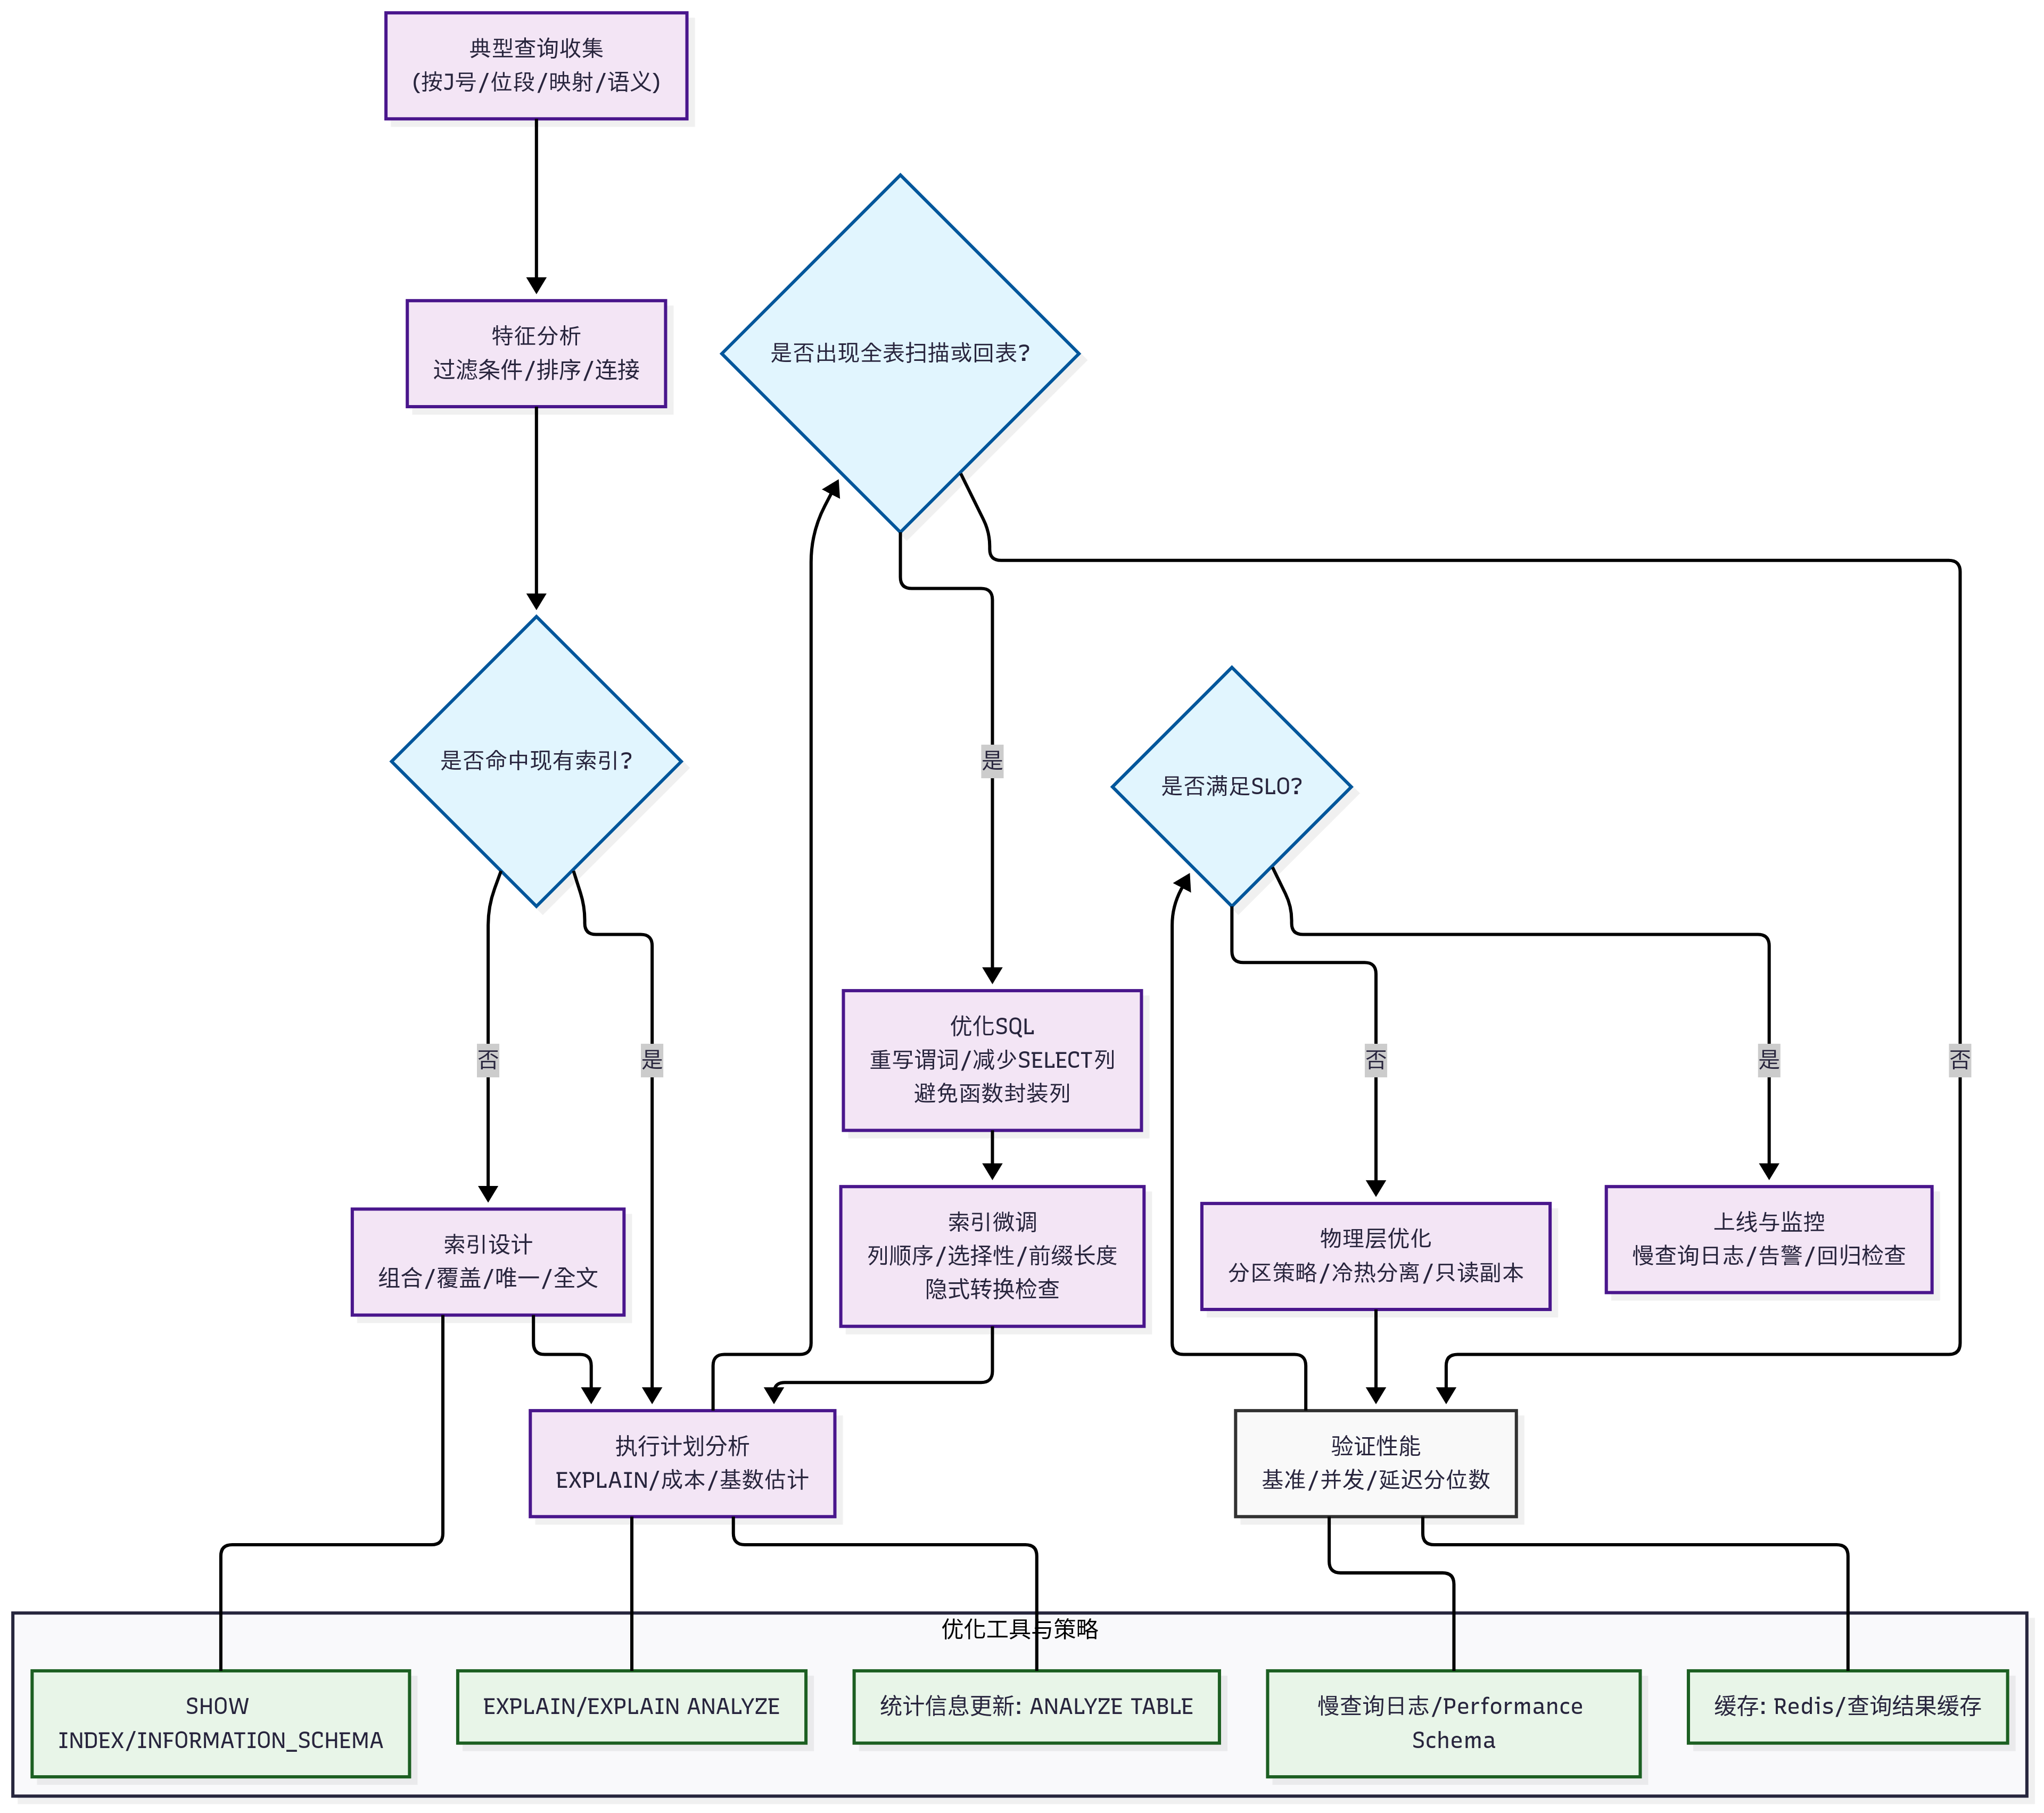
\includegraphics[width=0.8\textwidth,height=0.33\textheight,keepaspectratio]{chapters/fig-0/index-opt.png}
    \caption{索引与查询优化流程图}
    \label{fig_index_opt}
\end{figure}
以下为典型查询示例:

\begin{verbatim}
-- 查询某标准版本下 J3.x 系列消息
SELECT j_num, title
FROM message
WHERE std_id = '6016D' AND j_series LIKE 'J3.%';

-- 查询某消息的字段位段信息
SELECT start_bit, end_bit, dtype, unit
FROM field
WHERE message_id = 'UUID_xxx'
ORDER BY start_bit;

-- 查询某消息在 TTNT 链路下的映射规则
SELECT rule, confidence
FROM mapping m
JOIN linktype l ON m.link_id=l.link_id
WHERE m.message_id='UUID_xxx' AND l.name='TTNT';
\end{verbatim}

\subsection{查询优化策略}
在实验过程中,采用以下优化手段以提升整体查询性能:
\begin{itemize}
  \item \textbf{执行计划分析}:利用 \texttt{EXPLAIN} 命令分析 SQL 执行计划,调整索引与连接方式;
  \item \textbf{覆盖索引}:将高频查询所需字段放入同一索引,避免回表;
  \item \textbf{分区表设计}:按标准版本或消息类别分区存储,减少扫描范围;
  \item \textbf{缓存机制}:结合 Redis 等内存缓存,对高频查询结果进行缓存,降低数据库压力。
\end{itemize}

\subsection{性能评估}
在 MySQL 8.0 环境下,通过索引优化与缓存机制,百万级消息表的典型查询响应时间由秒级降低至百毫秒级,满足实时性要求。同时,跨链映射查询在并发 1000 级别下仍保持亚秒级延迟,证明了优化设计的有效性。

\section{数据一致性与完整性保障}

在战术数据链信息标准数据库的设计中,保证数据的一致性与完整性是系统能否稳定运行的核心要求。由于 {Link16} 消息涉及作战态势、指挥控制和火力协同等关键环节,任何数据丢失、错误或不一致都可能导致严重后果。因此,本系统在数据库层面和应用层面采取了多种措施,以确保数据质量与正确性。

\subsection{事务一致性与并发控制}
数据库采用事务管理机制,确保在多用户并发访问的情况下,消息的插入、更新和删除操作能够满足原子性、一致性、隔离性和持久性(ACID)原则。通过使用行级锁和多版本并发控制(MVCC),可以有效减少锁冲突,提升高并发条件下的数据一致性保障能力。

\subsection{完整性约束与规则定义}
在数据建模阶段,通过主键约束、外键约束和唯一性约束确保消息、字段和语义概念之间的逻辑关联不被破坏。例如,每一条 J 系列报文必须绑定唯一的消息编号,每个字段必须有合法的起止位范围和位长。这些约束条件保证了数据的结构完整性,避免了因手工输入或导入过程产生的逻辑错误。

\subsection{跨链互操作一致性}
随着多链融合和跨域作战的推进,数据链互操作性成为一致性保障的重要方面。系统在跨链路数据转换时,采用标准化的映射规则和中间件层协议(如 JREAP、SIMPLE),以避免在不同链路间传输数据时出现歧义和丢失。此外,结合多链融合技术研究成果,通过消息转发网关实现跨链信息的一致分发和控制。

\subsection{实时监控与异常处理}
为应对战术数据链的实时性需求,系统部署了实时数据校验与监控机制。通过比对消息的序列号、时间戳和校验字段,能够快速检测异常数据流,并触发回滚或重传机制。这种机制不仅提高了数据可靠性,也增强了在复杂电磁环境下的抗毁性和生存力。

\subsection{版本管理与可追溯性}
由于 {MIL-STD-6016} 等标准会不断修订升级,系统建立了版本控制机制,对不同标准版本下的消息定义进行分区存储与追踪。这样,在执行历史分析或跨版本互操作时,可以明确区分消息的版本背景,从而保证分析结果的一致性和可追溯性。

综上所述,本系统在数据一致性和完整性方面通过事务机制、约束规则、跨链互操作、实时监控和版本管理等多层措施构建了完备的保障体系。这不仅满足了高可靠性与高安全性的数据库应用需求,也为后续的联合作战和跨域互操作奠定了坚实基础。

\section{数据库安全与访问控制}

战术数据链信息标准数据库涉及敏感的军事信息,安全防护是系统设计的核心要求。本节将详细阐述数据库的安全架构设计,包括数据加密、访问控制、审计日志等安全机制。

\subsection{数据加密与存储安全}

系统采用多层次的数据加密策略,确保敏感数据在存储和传输过程中的安全性:

\textbf{存储层加密}:系统实现了透明数据加密(TDE)功能,对数据库文件进行全盘加密。采用AES-256加密算法,密钥通过硬件安全模块(HSM)进行管理。数据库备份文件同样采用加密存储,防止备份数据泄露。系统还支持字段级加密,对特别敏感的数据字段进行独立加密保护。

\textbf{传输层加密}:所有数据库连接都采用TLS 1.3协议进行加密传输,防止数据在传输过程中被窃取或篡改。系统实现了证书管理和验证机制,确保连接的可信性。对于高安全要求的场景,系统支持端到端加密,即使数据库管理员也无法查看明文数据。

\textbf{密钥管理}:系统建立了完善的密钥管理体系,包括密钥生成、分发、存储、使用、轮换和销毁的全生命周期管理。密钥采用分层管理策略,主密钥存储在HSM中,数据密钥通过主密钥加密后存储在数据库中。系统实现了自动密钥轮换机制,定期更新加密密钥,降低密钥泄露风险。

\subsection{访问控制与权限管理}

系统实现了基于角色的访问控制(RBAC)模型,确保用户只能访问其权限范围内的数据:

\textbf{用户认证}:系统支持多种认证方式,包括用户名密码认证、数字证书认证、生物特征认证等。对于高安全要求的场景,系统支持多因子认证(MFA),要求用户提供多种认证凭据。系统还集成了LDAP/AD等企业认证系统,支持单点登录(SSO)。

\textbf{权限控制}:系统实现了细粒度的权限控制,支持表级、行级、列级的访问控制。用户权限通过角色进行管理,每个角色具有特定的权限集合。系统支持权限继承和权限组合,允许用户具有多个角色的权限。权限控制还支持时间限制和IP限制,确保访问的安全性和可控性。

\textbf{数据脱敏}:系统实现了数据脱敏功能,对敏感数据进行匿名化处理。脱敏策略包括数据替换、数据屏蔽、数据泛化等方式。系统支持动态脱敏,根据用户权限动态决定是否显示敏感数据。脱敏规则可以自定义配置,满足不同场景的安全要求。

\subsection{审计日志与监控}

系统建立了完整的审计日志机制,记录所有数据库操作和访问行为:

\textbf{操作审计}:系统记录所有数据库操作,包括数据查询、插入、更新、删除等操作。审计日志包含操作时间、操作用户、操作类型、操作对象、操作结果等详细信息。系统还记录数据变更历史,支持数据变更的追踪和回滚。

\textbf{访问监控}:系统实时监控数据库访问行为,检测异常访问模式。监控指标包括访问频率、访问时间、访问来源、访问内容等。系统能够自动识别可疑的访问行为,如异常时间访问、大量数据导出、权限提升尝试等,并触发告警机制。

\textbf{安全告警}:系统建立了多层次的安全告警机制,包括实时告警、定期报告、紧急通知等。告警内容包括安全事件、性能异常、系统故障等。系统支持多种告警方式,包括邮件、短信、系统通知等。告警规则可以自定义配置,满足不同场景的监控需求。

\section{数据库备份与恢复}

数据库备份与恢复是确保数据安全性和系统可用性的重要保障。本节将详细阐述系统的备份策略、恢复机制和灾难恢复方案。

\subsection{备份策略设计}

系统采用多层次的备份策略,确保数据的安全性和可恢复性:

\textbf{全量备份}:系统定期进行全量备份,包括所有数据文件、日志文件和配置文件。全量备份采用增量备份技术,只备份发生变化的数据块,提高备份效率。备份文件采用压缩和加密存储,节省存储空间并保证安全性。

\textbf{增量备份}:系统支持增量备份和差异备份,只备份自上次备份以来发生变化的数据。增量备份大大减少了备份时间和存储空间,提高了备份效率。系统采用二进制日志(binlog)技术,实现精确的增量备份。

\textbf{实时备份}:系统实现了实时备份机制,通过主从复制技术将数据实时同步到备份服务器。实时备份不仅提供了数据保护,还支持读写分离和负载均衡。系统支持多级备份,包括本地备份、异地备份、云端备份等。

\subsection{恢复机制实现}

系统提供了多种数据恢复机制,满足不同场景的恢复需求:

\textbf{时间点恢复}:系统支持精确到秒的时间点恢复,能够将数据库恢复到任意时间点的状态。时间点恢复基于二进制日志和备份文件,通过重放日志操作实现数据恢复。系统提供了图形化的恢复界面,简化恢复操作流程。

\textbf{表级恢复}:系统支持表级恢复功能,能够恢复单个表或表分区,而不影响其他数据。表级恢复大大减少了恢复时间和系统影响,提高了恢复的灵活性。系统还支持行级恢复,能够恢复特定的数据行。

\textbf{跨平台恢复}:系统支持跨平台的数据恢复,能够在不同的操作系统和数据库版本间进行数据迁移。跨平台恢复基于标准的数据格式,确保数据的一致性和完整性。系统提供了自动化的迁移工具,简化跨平台恢复过程。

\subsection{灾难恢复方案}

系统建立了完整的灾难恢复方案,确保在重大灾难情况下的数据安全和业务连续性:

\textbf{异地容灾}:系统在异地建立了容灾中心,通过专线或VPN实现数据的实时同步。容灾中心具备完整的硬件和软件环境,能够在主中心故障时快速接管业务。系统支持自动故障切换和手动故障切换两种模式。

\textbf{业务连续性}:系统建立了业务连续性计划,包括故障检测、故障切换、业务恢复等流程。业务连续性计划明确了各种故障场景的处理流程和责任人,确保在故障发生时能够快速响应和恢复。

\textbf{恢复测试}:系统定期进行恢复测试,验证备份和恢复机制的有效性。恢复测试包括全量恢复测试、增量恢复测试、时间点恢复测试等。测试结果用于优化备份策略和恢复流程,提高系统的可靠性。

通过以上全面的安全防护和备份恢复机制,系统能够确保战术数据链信息标准数据库的安全性、可靠性和可用性,为军事应用提供坚实的数据保障。

\section{系统总体架构}

系统总体架构基于分层设计思想,结合数据库建模、后端服务和前端交互三大部分,形成了一个完整的、可扩展的体系结构。总体目标是实现对 {MIL-STD-6016} 及相关标准的消息存储、解析、查询与跨链互操作,支持研究人员、指挥员和运维人员的不同需求。

\subsection{分层设计}
系统总体架构设计是战术数据链信息标准数据库实现的核心,需要综合考虑技术选型、系统集成、性能优化和可扩展性等多个方面的需求。图\ref{fig_sys_arch}详细展示了系统总体架构的设计,该图通过架构图的形式清晰地描述了系统的整体结构和技术栈。图中可以看到,系统采用典型的"四层架构"模式,从下至上包括数据层、服务层、应用层和外部接口层。数据层采用MySQL关系数据库作为核心存储引擎,负责消息表、字段表、概念表、映射表及版本管理信息的持久化存储,通过事务机制和约束条件保证数据的一致性与完整性。服务层基于FastAPI框架实现RESTful接口,提供消息解析、数据校验、语义绑定和跨链映射等核心业务逻辑,支持异步处理和自动API文档生成。应用层包含前端交互模块,基于React与shadcn/ui组件库,提供消息检索、语义展示、态势可视化和统计分析等用户界面功能。外部接口层通过标准化API与外部仿真平台、作战指挥系统及跨链网关(如JREAP、TTNT)对接,支持系统的互操作性需求。这种分层架构设计不仅提高了系统的可维护性和可扩展性,还为不同层次的技术选型和性能优化提供了灵活性。

\begin{figure}[H]
    \centering
    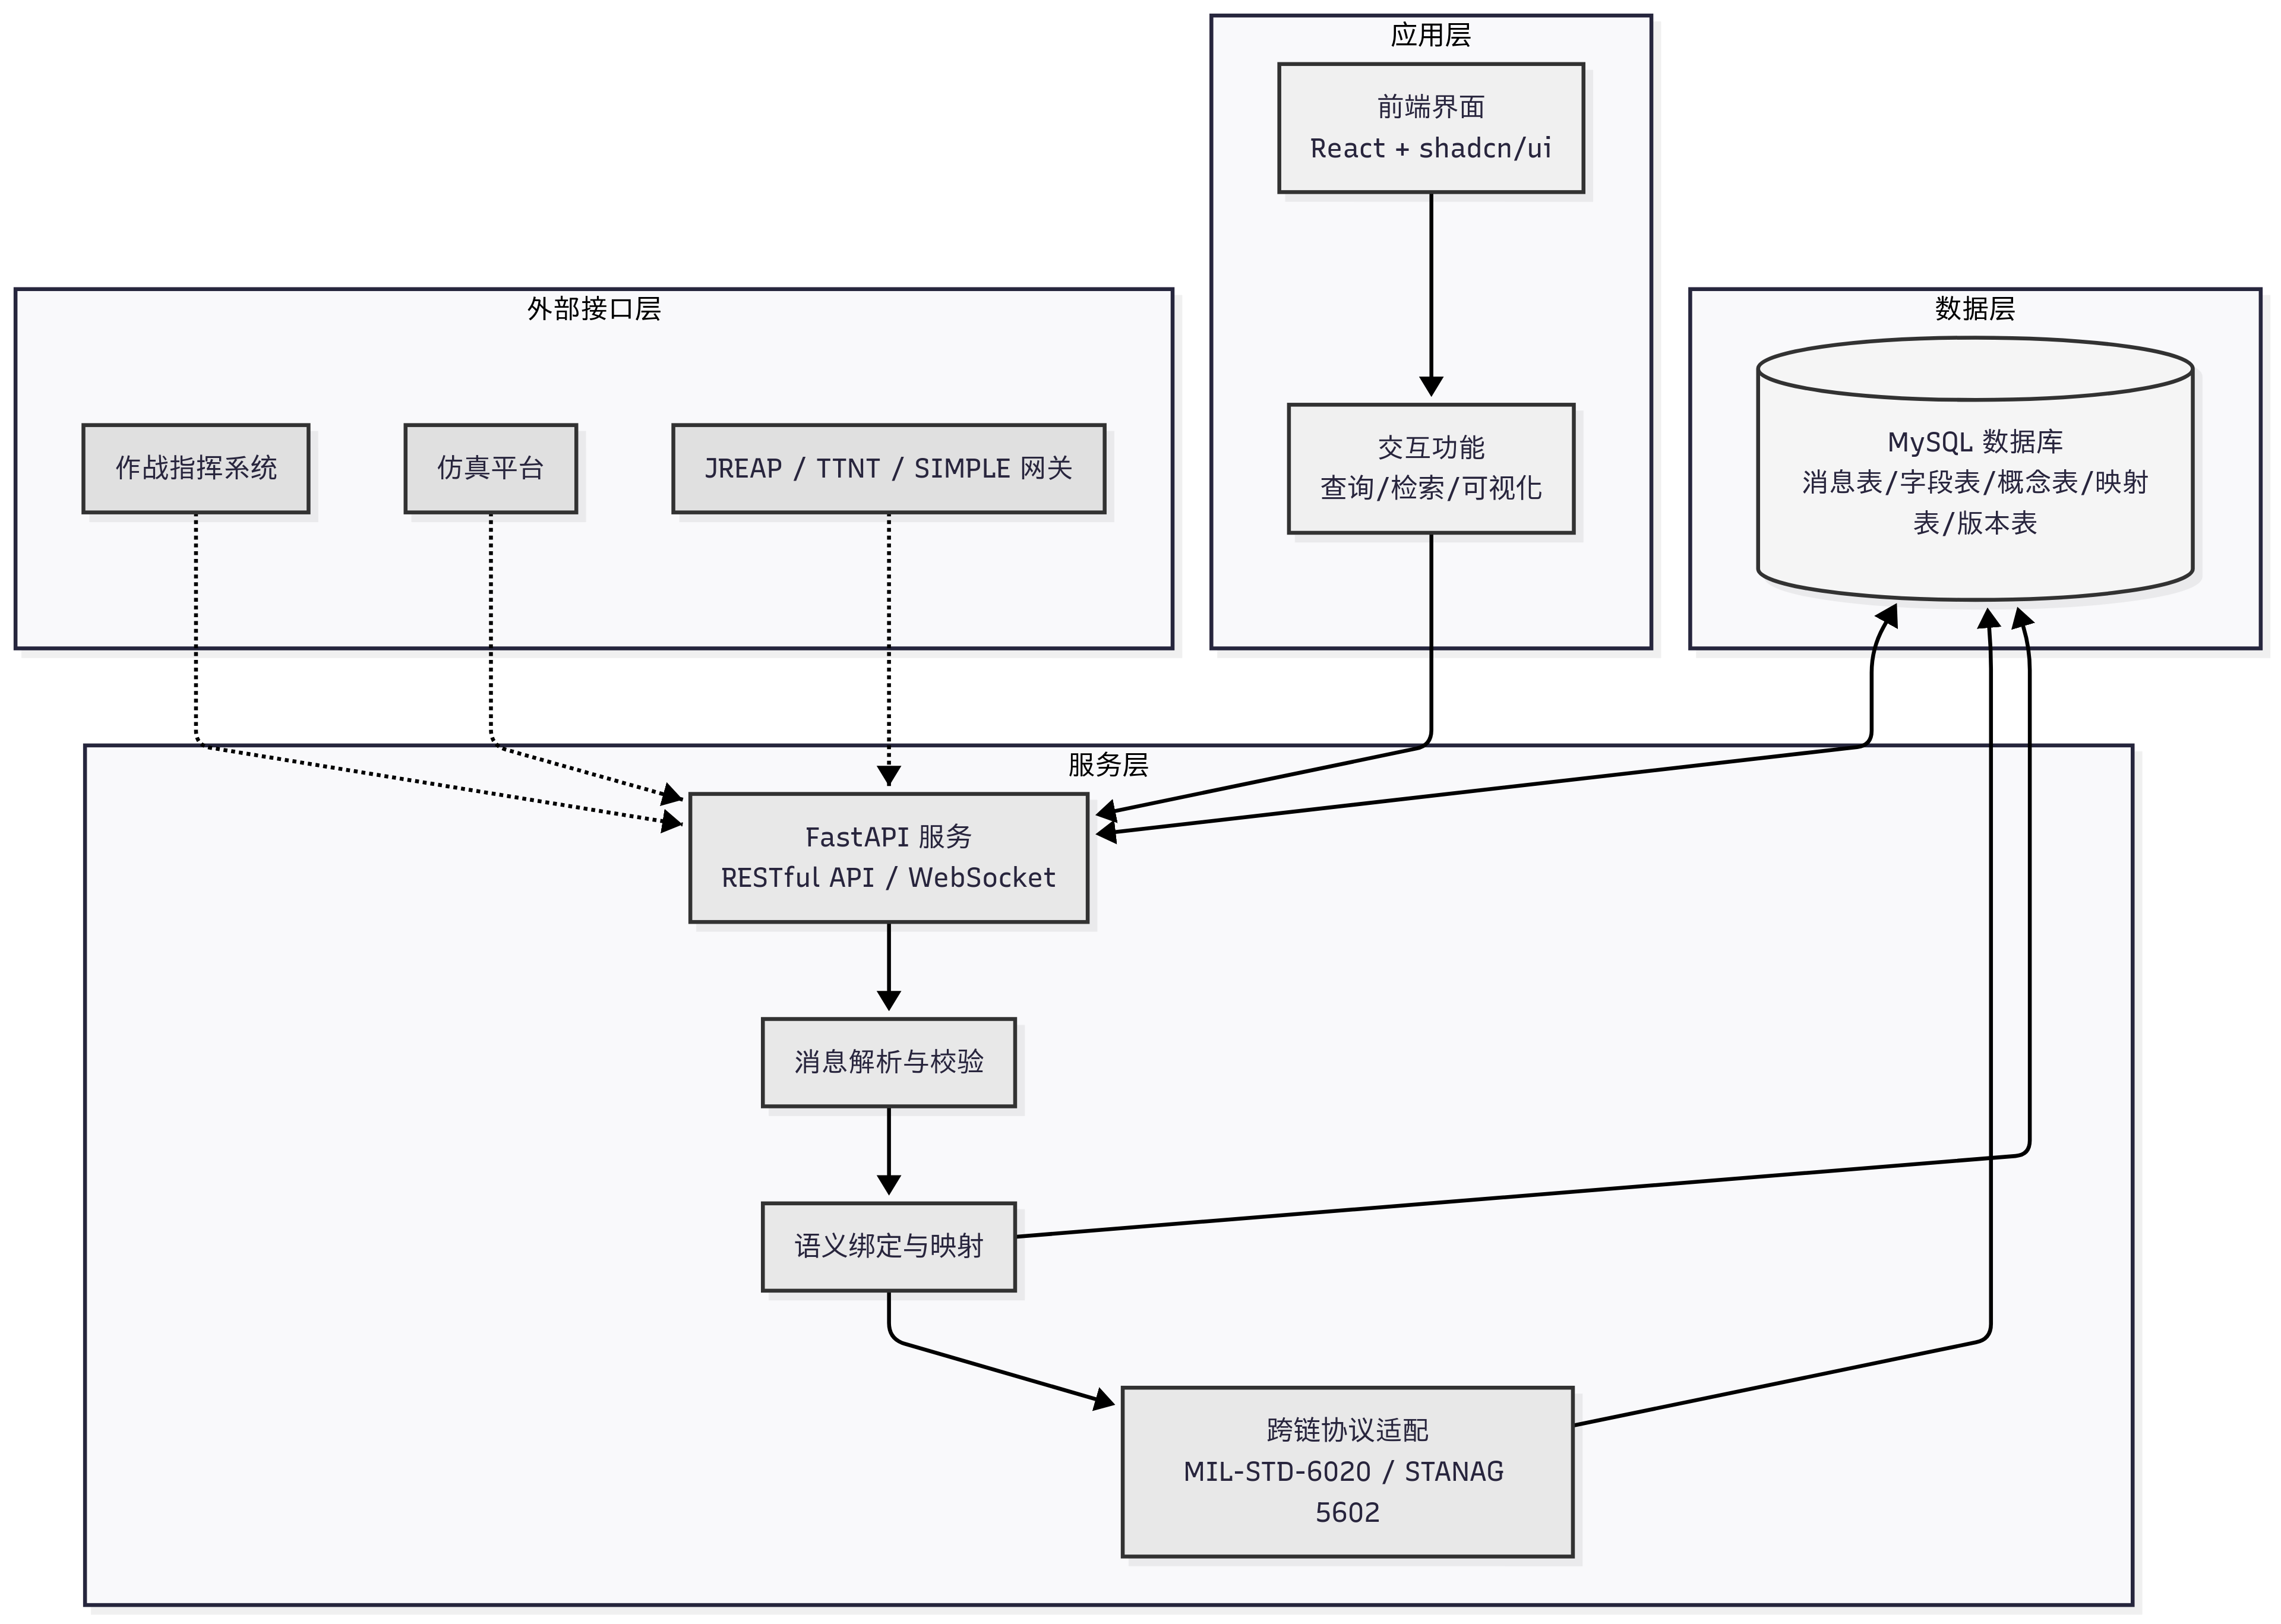
\includegraphics[width=0.8\textwidth,height=0.33\textheight,keepaspectratio]{chapters/fig-0/sys-arch.png}
    \caption{系统总体架构示意图}
    \label{fig_sys_arch}
\end{figure}
\begin{itemize}
  \item \textbf{数据层}:由 MySQL 数据库构成,存储消息表、字段表、概念表、映射表及版本管理信息,保证数据一致性与完整性;
  \item \textbf{服务层}:基于 FastAPI 实现 RESTful 接口,负责消息解析、数据校验、语义绑定和跨链映射逻辑;
  \item \textbf{应用层}:包含前端交互模块,基于 React 与 shadcn/ui,支持消息检索、语义展示、态势可视化和统计分析;
  \item \textbf{外部接口层}:通过标准化 API 与外部仿真平台、作战指挥系统及跨链网关(如 JREAP、TTNT)对接,支持互操作性需求。
\end{itemize}

\subsection{技术选型与实现}
在技术选型方面,系统采用了现代化的技术栈,确保高性能、可扩展性和易维护性:

\textbf{数据库技术}:选择 MySQL 8.0 作为主数据库,利用其事务处理能力、外键约束、全文索引等特性。同时,通过 Redis 实现缓存机制,提升查询性能。数据库设计遵循第三范式,确保数据一致性和完整性。

\textbf{后端技术}:采用 Python 3.10 + FastAPI 框架,利用其异步处理能力和自动 API 文档生成功能。FastAPI 基于 Pydantic 进行数据验证,确保接口的健壮性。同时,使用 SQLAlchemy 作为 ORM 框架,简化数据库操作。

\textbf{前端技术}:采用 React 18 + TypeScript 开发,使用 Vite 作为构建工具,提升开发效率。UI 组件库选择 shadcn/ui,基于 Radix UI 构建,提供现代化的用户界面。样式框架使用 TailwindCSS,实现响应式设计。

\textbf{部署技术}:采用 Docker 容器化部署,通过 Docker Compose 编排服务。使用 Nginx 作为反向代理和静态文件服务器,支持负载均衡和 SSL 终端。预留 Kubernetes 部署方案,支持微服务架构和自动扩缩容。

\section{后端架构设计}

后端架构采用模块化设计,将业务逻辑、数据访问和接口层分离,确保代码的可维护性和可扩展性。

\subsection{架构层次}
后端架构如图\ref{fig_fastapi_architecture} 所示。系统由路由层、服务层、数据库访问层三部分构成:  
\begin{enumerate}
  \item \textbf{路由层}:基于 FastAPI 的 APIRouter 定义接口,接收前端请求并进行参数校验;  
  \item \textbf{服务层}:实现业务逻辑,包括消息解析、数据清洗、语义绑定等;  
  \item \textbf{数据库层}:基于 SQLAlchemy 封装的 MySQL 数据访问模块,实现增删改查及索引优化。  
\end{enumerate}

后端服务架构设计是战术数据链信息标准数据库系统的核心组件,需要提供高性能、高可靠性的API服务来支撑前端应用和外部系统的数据访问需求。图\ref{fig_fastapi_architecture}详细展示了FastAPI后端服务架构的设计,该图通过架构图的形式清晰地描述了后端服务的内部结构和技术实现。图中可以看到,后端服务采用三层架构模式,包括路由层、服务层和数据库层。路由层基于FastAPI的APIRouter定义RESTful接口,负责接收前端请求、进行参数校验、身份认证和权限控制,同时提供自动API文档生成和接口测试功能。服务层实现核心业务逻辑,包括消息解析、数据清洗、语义绑定、跨链映射等功能模块,采用依赖注入和中间件机制,支持横切关注点的统一处理。数据库层基于SQLAlchemy ORM框架封装MySQL数据访问,提供异步会话机制、连接池管理、事务控制和查询优化等功能,在高并发场景下仍能保证数据一致性和系统性能。这种分层架构设计不仅提高了代码的可维护性和可测试性,还为系统的性能优化和功能扩展提供了良好的基础。

\begin{figure}[H]
    \centering
    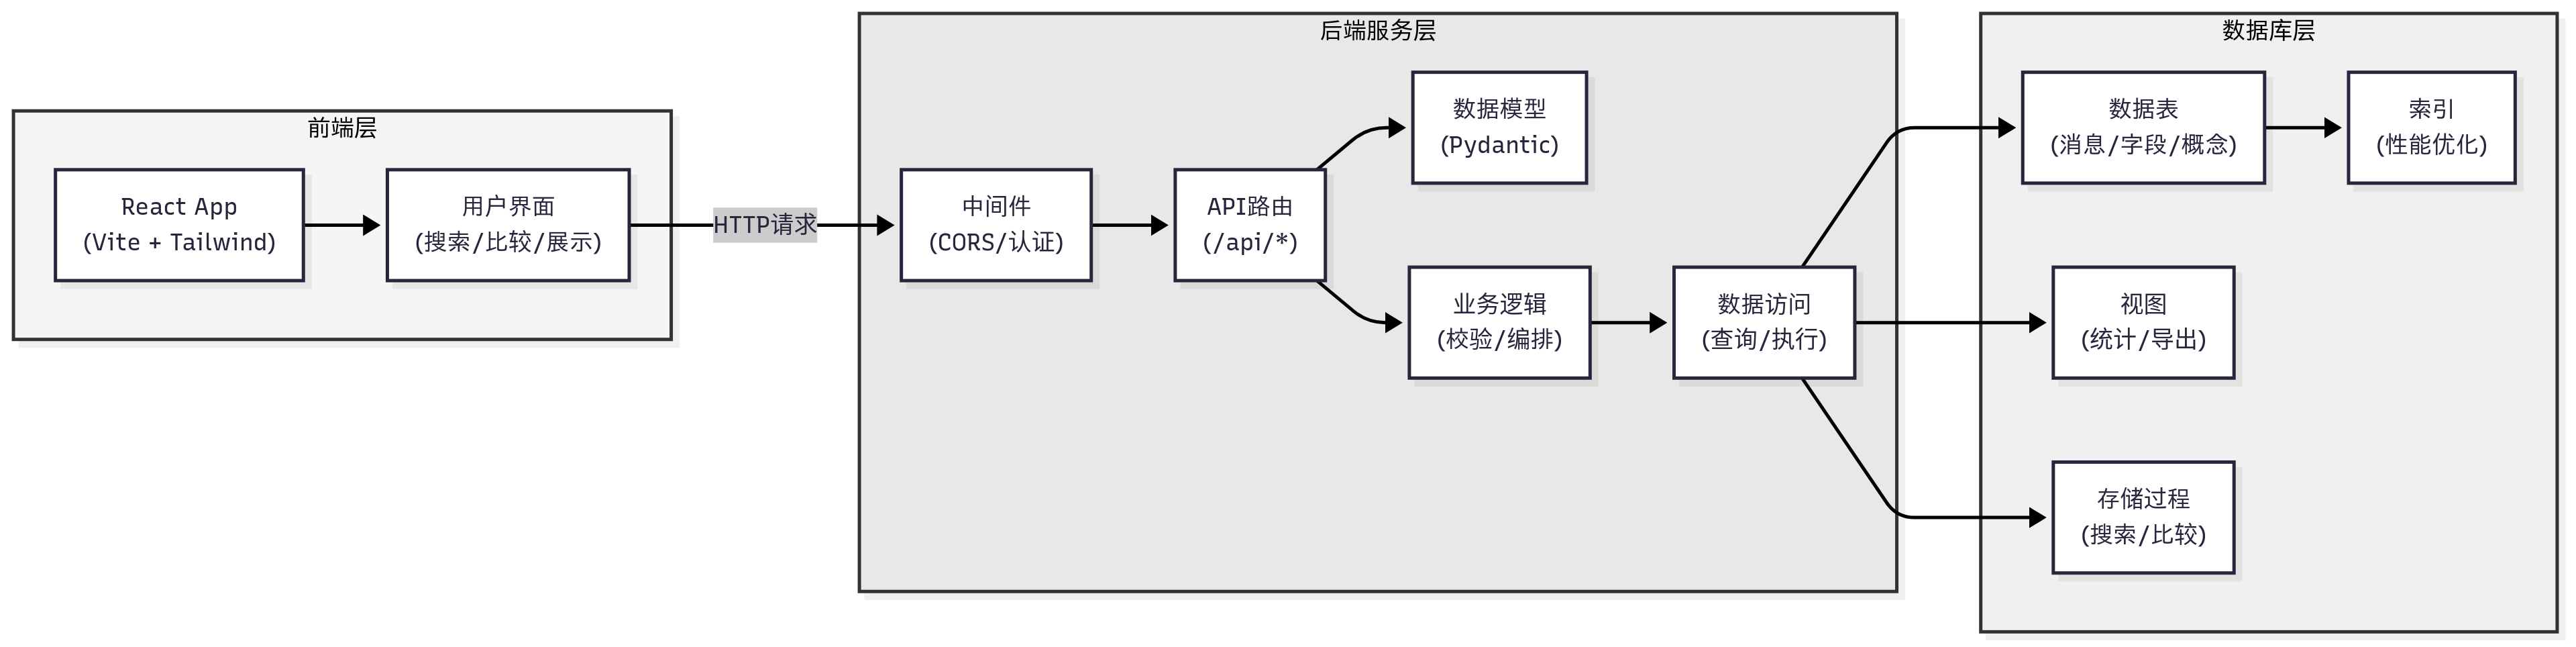
\includegraphics[width=0.8\textwidth,height=0.33\textheight,keepaspectratio]{chapters/fig-0/fastapi-architecture.png}
    \caption{FastAPI 后端服务架构示意图}
    \label{fig_fastapi_architecture}
\end{figure}

具体实现中,FastAPI 借助 Pydantic 完成输入输出模型的定义,保证消息体的完整性和合法性;  
数据库访问采用异步会话机制,在高并发场景下仍能保证数据一致性。  
同时,为适应战术数据链的实时性需求,后端提供了流式响应接口,用于处理仿真平台和实时作战环境中的高频消息。  

此外,后端还设计了跨标准消息的转发模块。例如,系统支持将 {Link16} 的 J 系列报文通过 {JREAP} 接口转发,实现卫星链路环境下的扩展通信能力,从而满足跨域互操作的需求。  

\subsection{核心接口设计}
系统提供了丰富的 RESTful API 接口,支持各种业务场景:

\textbf{搜索接口}:\texttt{/api/search} 支持关键词搜索、J 系列筛选和模糊匹配,返回结构化的搜索结果。接口支持分页查询,提高大数据量场景下的响应性能。

\textbf{比较接口}:\texttt{/api/compare} 实现跨标准版本的概念比较,支持按规范版本和消息类型进行聚合分析。接口返回详细的比较结果,包括字段数量、数据项数量等统计信息。

\textbf{绑定接口}:\texttt{/api/bind/field-to-di} 实现字段与数据项的语义绑定,支持自动概念生成和手动绑定调整。接口提供绑定关系的增删改查功能,支持批量操作。

\textbf{导出接口}:\texttt{/api/export} 支持多种格式的数据导出,包括 JSON、CSV 和 Excel 格式。接口支持按条件筛选导出,满足不同用户的数据需求。

\section{前端架构设计}

前端架构采用组件化设计,将界面功能模块化,提高代码复用性和维护性。

\subsection{技术栈选择}
前端技术栈的选择考虑了开发效率、用户体验和可维护性:

\textbf{React 框架}:选择 React 18 作为前端框架,利用其组件化开发模式和丰富的生态系统。React 的虚拟 DOM 机制提供了良好的性能,支持复杂的状态管理。

\textbf{TypeScript}:使用 TypeScript 进行类型检查,提高代码质量和开发效率。TypeScript 的静态类型系统能够减少运行时错误,提升代码的可维护性。

\textbf{状态管理}:使用 React Context 和 useReducer 进行状态管理,对于复杂的状态逻辑,预留了 Redux Toolkit 的集成方案。

\textbf{样式方案}:采用 TailwindCSS 作为样式框架,结合 shadcn/ui 组件库,实现现代化的用户界面。TailwindCSS 的原子化 CSS 方案提供了高度的定制性和一致性。

\subsection{组件架构}
前端组件架构采用分层设计,将组件按照功能层次进行组织:

\textbf{页面组件}:负责整个页面的布局和路由,包括搜索页面、比较页面、热门概念页面等。页面组件负责数据获取和状态管理。

\textbf{功能组件}:实现具体的业务功能,如搜索表单、结果展示、数据绑定等。功能组件具有良好的复用性,可以在不同页面中使用。

\textbf{基础组件}:提供基础的 UI 元素,如按钮、输入框、表格等。基础组件基于 shadcn/ui 构建,保证界面的一致性和可访问性。

\textbf{工具组件}:提供通用的工具功能,如数据格式化、错误处理、加载状态等。工具组件提高了代码的复用性和维护性。

\subsection{数据流设计}
前端数据流设计是战术数据链信息标准数据库系统用户界面的核心架构,需要确保数据在组件间的正确传递和状态的一致性管理。图\ref{fig:frontend-dataflow}详细展示了前端数据流与视图切换的设计,该图通过数据流图的形式清晰地描述了前端应用的数据流向和组件交互模式。图中可以看到,系统采用单向数据流模式,确保数据的一致性和可预测性。数据流从用户交互开始,通过事件处理机制触发状态更新,状态变化驱动视图重新渲染,形成完整的数据循环。用户交互层包括搜索表单、筛选条件、操作按钮等界面元素,用户的操作通过事件处理器转换为相应的动作。状态管理层采用React的useState和useContext等Hook机制,集中管理应用的状态数据,包括搜索结果、用户偏好、系统配置等。数据获取层通过API调用从后端服务获取数据,采用异步处理机制,支持加载状态和错误处理。视图渲染层根据状态数据动态渲染界面组件,包括搜索结果列表、数据表格、图表展示等。这种单向数据流设计不仅提高了应用的可维护性和可调试性,还确保了数据状态的一致性和用户界面的响应性。

\begin{figure}[H]
  \centering
  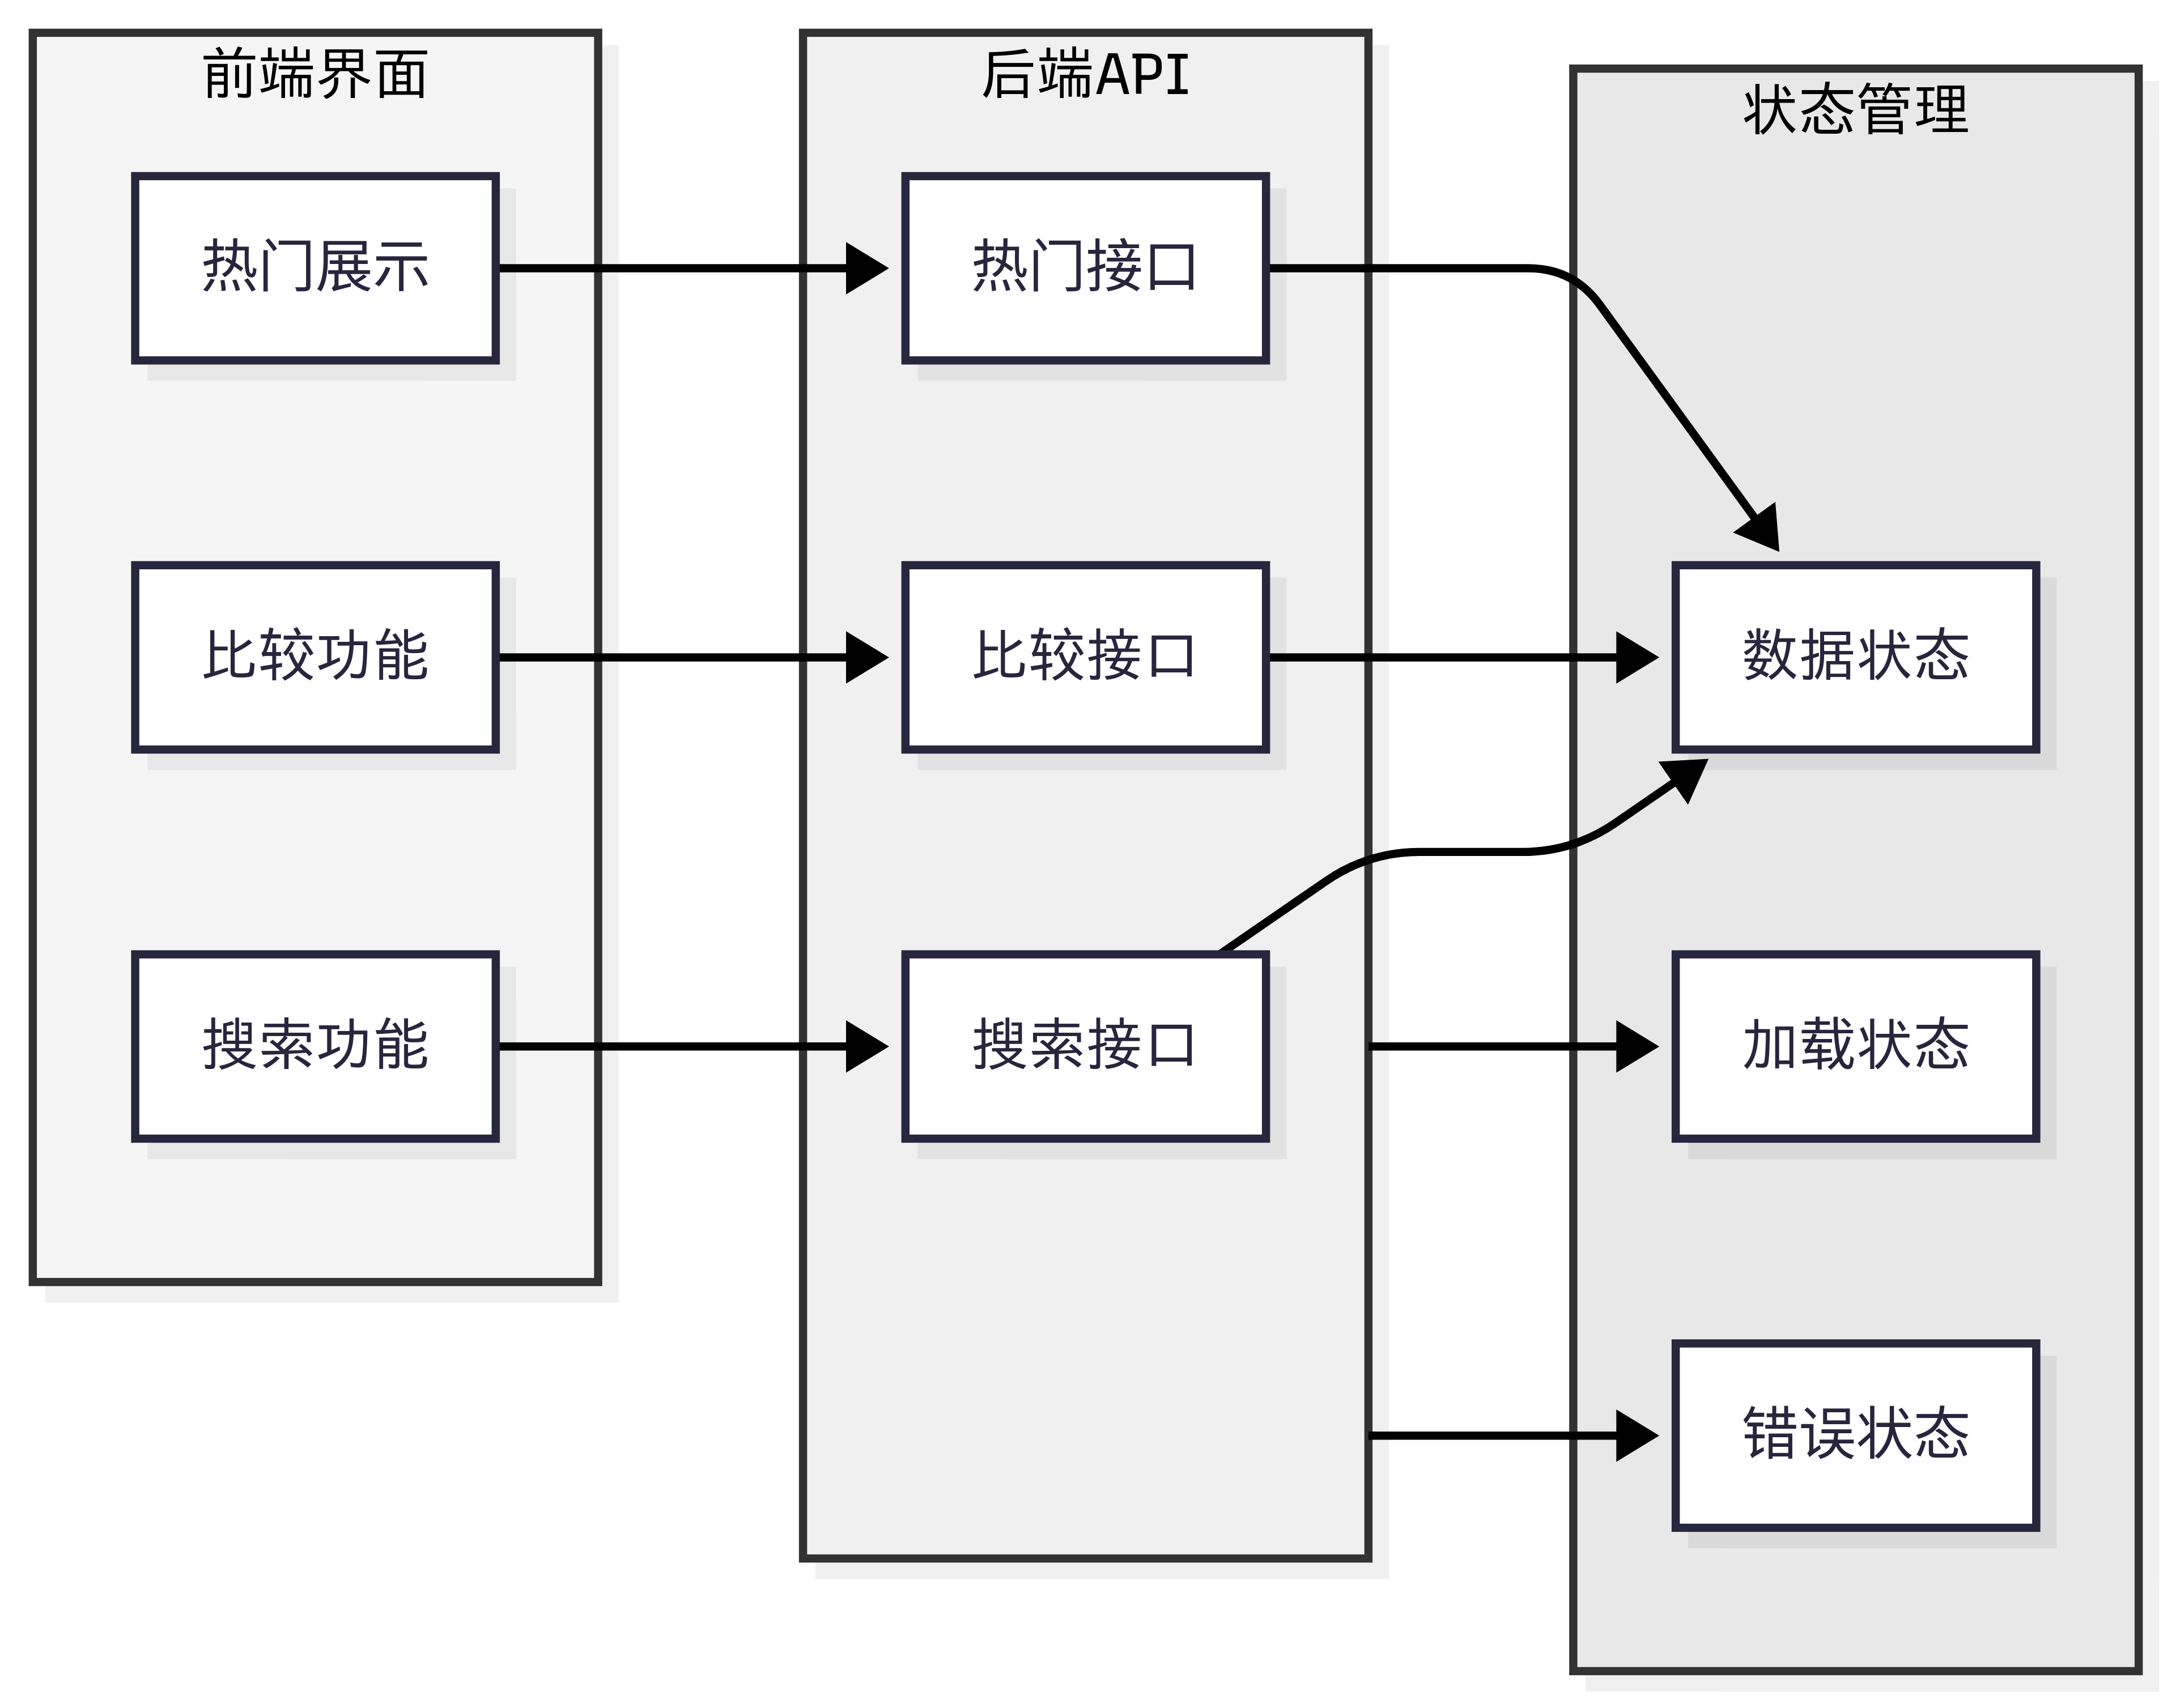
\includegraphics[width=0.8\textwidth]{chapters/fig-0/frontend-dataflow.png}
  \caption{前端数据流与视图切换示意图}
  \label{fig:frontend-dataflow}
\end{figure}

\textbf{数据获取}:通过自定义 Hook 封装 API 调用,实现数据的获取和缓存。Hook 提供了加载状态、错误处理和数据刷新功能。

\textbf{状态管理}:使用 React Context 管理全局状态,包括用户信息、搜索历史、主题设置等。状态更新通过 reducer 函数进行,确保状态变更的可预测性。

\textbf{视图更新}:组件根据状态变化自动更新视图,实现响应式的用户界面。视图更新采用虚拟 DOM 机制,提高渲染性能。

\subsection{主要组件与样式}
系统主要使用以下组件:
\begin{itemize}
  \item \textbf{输入与筛选}:Input、Select、Switch 组件用于关键词、J 系列、模糊匹配条件输入。
  \item \textbf{表格展示}:Table 组件提供"概念/字段"与"按字"两种结果视图切换,支持位段 Badge 高亮。
  \item \textbf{反馈机制}:Badge、错误提示卡片、Loading 动画保证用户在网络中断或后端不可用时仍能获得清晰提示。
  \item \textbf{导航与布局}:Tabs 组件实现功能模块切换,Card 组件提供内容分组,整体采用响应式布局适配不同屏幕尺寸。
\end{itemize}

样式方面,系统采用现代化的设计语言,包括:
\begin{itemize}
  \item \textbf{色彩方案}:使用语义化的颜色系统,包括主色调、辅助色和状态色,确保界面的视觉一致性。
  \item \textbf{字体系统}:采用系统字体栈,确保在不同操作系统下的良好显示效果。字体大小和行高经过精心设计,提高可读性。
  \item \textbf{间距系统}:使用 TailwindCSS 的间距系统,确保界面元素之间的视觉平衡。
  \item \textbf{动画效果}:使用 CSS 过渡和动画,提供流畅的用户交互体验。
\end{itemize}

通过以上全面的架构设计,系统实现了从数据库到前端界面的完整技术栈,为战术数据链信息标准的管理和应用提供了坚实的技术基础。
